% !TeX program = xelatex
\documentclass[12pt,a4paper,fontset=windows]{ctexart}
\setCJKfamilyfont{zhsong}{SimSun}[AutoFakeBold=1.8]
\setCJKfamilyfont{zhhei}{SimHei}[AutoFakeBold=1.8]
% ── 中文标点禁则：行末半角 + 禁止标点出现在行首 ──
\xeCJKsetup{PunctStyle=hangmobanjiao}

% ── 页面布局 ──
\usepackage[top=2.54cm, bottom=2.54cm, left=3.18cm, right=3.18cm]{geometry}

% ── 数学 ──
\usepackage{amsmath, amssymb}
\usepackage{physics}

% ── 图表 ──
\usepackage{graphicx}
\usepackage{caption}
\usepackage{subcaption}
\usepackage{booktabs}
\usepackage{array}
\usepackage{tabularx}
\usepackage{float}
\usepackage{multirow}

% ── 行距 ──
\usepackage{setspace}
\setstretch{1.25}
\setlength{\emergencystretch}{2em}

% ── 页眉页脚 ──
\usepackage{fancyhdr}
\pagestyle{fancy}
\fancyhf{}
\fancyhead[C]{\songti\zihao{5} 物理创新实验报告}
\fancyfoot[C]{\songti\zihao{-5} \thepage}
\renewcommand{\headrulewidth}{0.4pt}
\setlength{\headheight}{15pt}

% ── 超链接 ──
\usepackage[hidelinks]{hyperref}
\hypersetup{colorlinks=true, linkcolor=black, citecolor=black}

% ── 首行缩进 ──
\usepackage{indentfirst}

\ctexset{
  section = {
    format = \heiti\zihao{-3}\centering,
    beforeskip = 1.5ex plus 0.3ex minus 0.2ex,
    afterskip = 1.0ex plus 0.2ex minus 0.2ex,
  },
  subsection = {
    format = \heiti\zihao{-4}\raggedright,
    beforeskip = 1.0ex plus 0.2ex minus 0.2ex,
    afterskip = 0.8ex plus 0.2ex minus 0.2ex,
  },
  subsubsection = {
    format = \heiti\zihao{-4}\raggedright,
    beforeskip = 0.8ex plus 0.2ex minus 0.2ex,
    afterskip = 0.5ex plus 0.1ex minus 0.1ex,
  },
}

\graphicspath{{figures/}}
\captionsetup{font=small, labelsep=quad}

\begin{document}

% ============================================================
% 封面
% ============================================================
\begin{titlepage}
\begin{center}
\vspace*{2.5cm}

{\heiti\zihao{2} 大连理工大学}

\vspace{0.8cm}

{\heiti\zihao{-0} 物理创新实验报告}

\vspace{3.0cm}

\begin{center}
\renewcommand{\arraystretch}{1.8}
\large
\begin{tabular}{>{\heiti}l<{\songti}>{\large\songti}c}
  实验题目：& \underline{\makebox[11.1cm]{基于原子力显微镜的光盘表面沟槽形貌测量}} \\[0.6cm]
  学院（系）：& \underline{\makebox[11.1cm]{物理学院}} \\[0.6cm]
  专\hspace{2em}业：& \underline{\makebox[11.1cm]{应用物理学}} \\[0.6cm]
  完成日期：& \underline{\makebox[11.1cm]{\today}} \\
\end{tabular}
\end{center}
\end{center}
\end{titlepage}

% ============================================================
% 摘要
% ============================================================
\setcounter{page}{1}
\section*{\heiti\zihao{-3}\centering 摘要}

\vspace{0.3cm}

\songti\zihao{-4}
\setstretch{1.25}

本实验用接触模式原子力显微镜（CSPM5500，$10\,\mu\mathrm{m}\times10\,\mu\mathrm{m}$ 视场，$1024\times1024$ 点）测量了三张不同光盘的表面形貌，对形貌、误差信号与横向力三个通道的数据建立了完整的离线处理链，并给出沟槽周期、峰谷深度与面粗糙度的定量结果。三张光盘的沟槽周期分别为 $2170\pm4$、$2143\pm7$ 与 $1090\pm2$~nm（$\pm$ 为行间四分位半宽），逐行峰谷深度分别为 55.2、60.4 与 93.4~nm，整平后面均方根高度 $S_q$ 为 20.26、19.94 与 31.02~nm。前两张光盘倾角修正后的周期相差 0.25\%，在本数据的精度内可视为同一规格；以 CD 标准道距 1600~nm 为参照反推的快扫轴横向标定因子为 1.34，据此第三张光盘修正后的周期为 792~nm，与 DVD 道距 740~nm 相差 7.0\%。按此标定，三张光盘对应两张 CD 类与一张 DVD 类；该判断以盘片道距等于标称值为前提，标定因子由道距反推得到，并非独立测得。图像中条纹相对慢扫方向（$y$ 轴）存在 $8.1^\circ$ 与 $-13.2^\circ$ 的倾斜，直接沿慢扫方向平均时条纹在平均中相互抵消（第三张光盘的平均剖面峰谷由 88.6~nm 降至 8.1~nm），按倾角对齐后峰谷恢复到 88.6~nm。原始图像行均值序列的标准差不超过 0.06~nm，相邻行均值差的平均绝对值不超过 0.004~nm，三组数据均未见扫描线伪迹；误差信号与横向力通道对同一沟槽结构给出同向响应。本实验还给出扫描器横向标定的不确定度对周期测量的影响，以及探针卷积使深度读数偏小的量级估计；并以 CD 与 DVD 的标准道距为约束作贝叶斯联合拟合，给出横向标定因子的后验 1.34--1.43，并指出标定因子与道距在数据中不可分离。

\vspace{0.5cm}
\noindent{\heiti\zihao{-4}\bfseries 关键词：}\songti\zihao{-4}原子力显微镜；光盘沟槽；粗糙度；横向标定；探针卷积

\newpage

% ============================================================
% 引言
% ============================================================
\section{引言}

\subsection{扫描探针显微镜的发展与分类}

扫描探针显微镜（scanning probe microscope, SPM）以一根尖锐探针在样品表面上方作栅格扫描，通过记录探针与样品之间的局域相互作用成像，其分辨率不取决于波长，而取决于探针尖端的尺寸与探针—样品间距的控制精度。1982 年，Binnig、Rohrer、Gerber 等报道了利用金属探针与导电样品之间的隧道电流获得表面原子尺度形貌成像的工作，即扫描隧道显微镜（scanning tunneling microscope, STM）\cite{binnig1982}。STM 要求样品与探针之间能够维持稳定的隧道电流，因而样品必须导电，绝缘体与多数生物样品无法直接测量。

1986 年，Binnig、Quate 与 Gerber 以探测微悬臂的形变代替隧道电流，把测量的物理量从电流换成力，提出了原子力显微镜（atomic force microscope, AFM）\cite{binnig1986}。这一改动的意义在于：探针与样品之间的相互作用力对样品的导电性没有要求，AFM 因而把 SPM 的适用范围从导体、半导体扩展到绝缘体，也使 SPM 从表面物理的实验手段变成材料、化工、生物、微电子等领域通用的形貌表征工具。

扫描探针显微镜是一个由探针—样品局域相互作用成像的家族：把隧道针尖换成力敏感微悬臂即得原子力显微镜，换成近场光学探针、微热计等则衍生出多种扫描探针显微镜\cite{giessibl2003}。按所探测的物理量，常用的 SPM 包括探测隧道电流的 STM、探测针尖—样品作用力的 AFM、探测横向（摩擦）力的横向力显微镜（lateral force microscope, LFM）、以两遍扫描探测磁性相互作用的磁力显微镜（magnetic force microscope, MFM）、探测静电梯度的静电力显微镜（electrostatic force microscope, EFM）、把光场限制在近场从而突破衍射极限的扫描近场光学显微镜（scanning near-field optical microscope, SNOM），以及在扫描的同时记录隧道电流—电压曲线、给出局部电学性质的扫描隧道谱\cite{mironov2004}。本文的测量对象是形貌，同时记录了误差信号与横向力两路信号，后者即 LFM 意义上的摩擦力信号：横向力显微镜自 1987 年起即为研究原子尺度摩擦的手段\cite{giessibl2003}。

\subsection{原子力显微镜的工作模式}

AFM 的核心是一枚末端带有针尖的微悬臂。针尖与样品距离较近时，两者之间的范德华力、静电力与短程排斥力随距离急剧变化；悬臂受力的弯曲量由光杠杆法测量：一束激光聚焦在悬臂背面，反射光落在四象限光电探测器（position-sensitive detector, PSD）的中心，悬臂的角偏转使光斑在探测器中心附近平移，其位移由各扇区的差分电流给出\cite{mironov2004,meyer1988}。四象限探测器的两路差分信号分别给出法向形变与扭转，即
\begin{equation}
\Delta I_Z = (\Delta I_1+\Delta I_2)-(\Delta I_3+\Delta I_4),\qquad
\Delta I_L = (\Delta I_1+\Delta I_4)-(\Delta I_2+\Delta I_3),
\label{eq:quad}
\end{equation}
式~\eqref{eq:quad} 中 $\Delta I_i$ 为各扇区电流相对参考值的变化；$\Delta I_Z$ 正比于法向力引起的弯折，$\Delta I_L$ 对应横向力（摩擦力）引起的扭转\cite{mironov2004}。反馈回路以这个位移为输入，通过压电扫描器的 $z$ 向伸缩把位移维持在设定值，于是 $z$ 向电压的变化就记录了表面高度。

按针尖与样品的接触状态，AFM 有三种常用工作方式。接触模式（contact mode）使针尖始终与样品接触，恒力模式下反馈回路保持悬臂的弯折量恒定，于是 $z$ 向电压的变化即记录表面高度；其缺点是针尖与样品直接机械作用，常导致针尖磨损或样品表面损伤，对有机与生物等软样品基本不适用\cite{mironov2004}。轻敲模式（tapping mode，也称间歇接触模式）使悬臂在自由共振频率附近受激振动，振幅约 10--100~nm，仅在下摆段与样品接触，反馈量是振幅\cite{mironov2004}；由于只需把最大针尖—样品作用力压到较低水平即可避免不可逆形变，它适合软样品与生物样品\cite{garcia2002}。非接触模式（non-contact mode）使悬臂以约 1~nm 的小振幅在吸引力梯度高的区域受激振动，探测的是力梯度；但从振幅与相位的变化中提取信号要求反馈具有很高的灵敏度与稳定性，实际测量中更常用轻敲（半接触）模式\cite{mironov2004}。本实验的测量对象是光盘数据面一侧的预刻沟槽形貌，其峰谷起伏在数十纳米量级，选用接触模式以获得较强的形貌与误差信号对比。

三种模式之外，AFM 还有若干辅助成像方式：抬起模式（lift mode）在每一扫描行结束后把针尖抬高到固定高度再回扫，用于 MFM/EFM；力调制模式在扫描的同时对悬臂施加小幅高频调制，通过形变幅度的变化反映表面刚性差异；纳米加工模式则利用针尖与样品之间的强相互作用或电场在表面刻写结构\cite{manual_cspm}。

\subsection{光盘的结构、记录原理与格式演进}

光盘以聚碳酸酯（polycarbonate, PC）圆盘为基片，通过注塑把信息坑（pit）或预刻沟槽（pre-groove）复制在基片表面，再逐层覆盖功能膜。以可记录光盘 CD-R 为例，自读取面（激光入射面）向内部依次为：聚碳酸酯基片（厚 1.2~mm，提供机械强度并承载预刻沟槽）、有机染料记录层（花菁类染料，是记录介质，厚度在百纳米量级\cite{kim1997}）、反射层（金或银合金，提供高反射率）、保护层（紫外固化胶，防止反射层氧化与机械划伤）、印刷层（标签，便于书写与识别）。激光自读取面入射，先穿过基片再到达染料层。基片上的预刻沟槽是螺旋状的连续槽，槽与槽之间的平坦区域称为岸（land）；沟槽既提供记录时激光的跟踪基准，也界定染料涂布的区域。

CD-R 的记录过程是热化学过程\cite{kim1997}：聚焦激光使染料层发生热致变化，染料部分分解，形成永久标记，标记区的反射率降低。读取时用较低功率的激光照射，光电探测器接收反射光，反射率的差异被解调为数字信号。这一点与压制式 CD-ROM 不同：后者的信息坑在注塑时就已成型在基片上，而 CD-R 的“坑”是写入后才产生的，因此 CD-R 的记录层必须是可发生不可逆变化的材料。由于染料层位于基片之上、反射层之下，记录前后标记的几何高度会发生变化，这一变化在 AFM 形貌图上表现为沿轨道的局部凸起或凹陷。

跟踪信号由沟槽本身提供。激光束在沟槽上偏离中心时，反射光的分布发生不对称变化，四象限探测器的差动信号（推挽信号）给出偏离方向与大小，伺服系统据此把光斑锁在沟槽中心。为保证跟踪与转速的基准，CD-R 的沟槽中心线并非直线，而是以 22.05~kHz 的载波频率左右摆动（wobble）；载波经 FM 调制（频偏约 1~kHz）后携带绝对时间信息，称为 ATIP（absolute time in pre-groove）。写入时，记录机由 ATIP 的时间码确定写入位置、由载波频率作为线速度（转速）的基准\cite{ecma394}。

各代光盘的差别主要体现在三个参数：激光波长、物镜数值孔径与道距。缩短波长与增大数值孔径可使聚焦光斑变小，从而缩小道距与最小记录符长度，提高面密度。表~\ref{tab:format} 列出主要格式的典型参数，其中 CD 与 DVD 的激光波长、数值孔径与道距取自 ECMA-130 与 ECMA-267，蓝光取自 Blu-ray 白皮书，HD DVD 的参数仅有二手来源；容量与最小记录符长度为格式的通用标称值，其中 CD 的 0.83~$\mu$m 由 1.2~m/s 扫描速度与 4.3218~Mbit/s 信道位率按 3T 换算，DVD 的 0.40~$\mu$m 由 133.3~nm 信道位长按 3T 换算\cite{ecma130,ecma267,bda2004}。对本实验而言，这些参数的意义在于：道距决定了 AFM 视场内可见的沟槽条数，10~$\mu$m 的视场在 CD 类光盘上应看到约 6 条、在 DVD 类上约 13 条、在蓝光上约 31 条；沟槽深度则决定了形貌图与横向力图的对比度。

\begin{table}[H]
\centering
\caption{主要光盘格式的典型参数}
\label{tab:format}
\small
\setstretch{1.0}
\begin{tabular}{@{}lccccc@{}}
\toprule
格式 & 激光波长/nm & 数值孔径 & 道距/$\mu$m & 最小坑长/$\mu$m & 单层容量 \\
\midrule
CD / CD-R & 780 & 0.45 & 1.60 & 0.83 & 650--700 MB \\
DVD / DVD-R & 650 & 0.60 & 0.74 & 0.40 & 4.7 GB \\
HD-DVD & 405 & 0.65 & 0.40 & 0.20 & 15 GB \\
Blu-ray & 405 & 0.85 & 0.32 & 0.15 & 25 GB \\
\bottomrule
\end{tabular}
\end{table}

用 AFM 检测光盘表面在国内外均有报道：早期工作关注基片的沟槽几何、染料旋涂均匀性对 CD-R 制造质量的影响，并观测了记录前后的标记形貌\cite{sunjielin2001}；国内亦有对光盘与 CD/DVD 表面微结构（凹坑深度、道间距）的系统测量\cite{yanyg2005,sunzhi2006}，并对形貌像的典型失真与伪迹作出分类\cite{lipeng2016}。

上述道距与最小坑长是格式标准规定的标称值，实际盘片存在公差；而 AFM 测得的表观周期还额外受扫描器标定的影响。本文第~\ref{sec:calib} 节给出这两者在本次测量中的区分依据。

\subsection{本实验的目的与内容}

本实验用接触模式 AFM 测量三张光盘的表面，内容包括采集形貌、误差信号与横向力三路图像，观察同一表面在不同物理量上的响应；对形貌图作消除扫描线、面整平与对比度调整等处理，比较处理前后参数的变化；定量给出沟槽周期、峰谷深度与面粗糙度，并与格式标准的标称值对照，据此讨论扫描器横向标定的状态；识别并定量评估扫描线、条纹倾斜、探针卷积等常见伪迹，说明其对测量结果的影响量级。


% ============================================================
% 实验原理与方法
% ============================================================
\section{实验原理与方法}

\subsection{扫描与反馈参数}

扫描由压电扫描器带动针尖作栅格运动：快扫方向（本文的 $x$）每行往返一次，慢扫方向（本文的 $y$）逐行推进，视场由软件设定的扫描范围决定。反馈回路由参考点、比例增益、积分增益与参考增益四个参数决定（参考增益用上一行的数据预测当前行的形貌，本实验取 0，未启用）。参考点给出反馈要维持的相互作用大小（软件中记为 Ref，本实验取 0.30），比例增益决定对当前误差的补偿快慢，积分增益补偿累积的系统误差\cite{manual_cspm}；比例与积分增益越大反馈越灵敏，过大时引入振荡。扫描频率定义为探针在快扫方向每秒往返的行数，本实验取 1.0~Hz，处于该仪器推荐的 1.0--2.0~Hz 区间。在固定的扫描频率下，扫描范围越大，针尖在样品表面的线速度越高，反馈跟踪形貌变化的时间余量越小。

仪器同时记录三路信号。形貌信号是反馈回路为维持参考点而施加的 $z$ 向电压，按满量程高度换算为高度；误差信号是实际偏转与参考点之差（软件中记为“探针起伏”），正比于表面高度沿扫描方向的变化率，在平台处趋于零、在槽壁处出现极值，对边缘与高频形貌比形貌通道敏感；横向力信号来自悬臂的扭转，反映针尖与样品之间的摩擦力，在沟槽两侧的上坡与下坡段方向相反。三路信号由同一支探针、同一行程同时采集，因而可以逐点对照。

\subsection{实验装置与样品}

仪器为本原纳米仪器 CSPM5500 扫描探针显微镜（软件版本 V4.60，序列号 CSPM5500-200906A），配 S8163 扫描器。扫描器的最大扫描范围由四个方向伸缩系数中的最小值决定，手册给出的关系为
\begin{equation}
L_{\max} = \min\left(k_{X}^{\text{fast}},\,k_{Y}^{\text{fast}},\,k_{X}^{\text{slow}},\,k_{Y}^{\text{slow}}\right)\times 360~\mathrm{V},
\label{eq:maxscope}
\end{equation}
其中伸缩系数的单位为 $\mathrm{nm/V}$。本机四个方向的伸缩系数取自软件扫描器标定页，分别为 251.087、251.943、318.454 与 317.546~nm/V；代入式~\eqref{eq:maxscope} 得 $L_{\max}=90\,391~\mathrm{nm}$，与同一页的 Max Scope 读数一致，说明扫描器参数设置自洽。

样品为三张成品光盘，依次记为 cd1、cd2 与 cd3，型号未作记录。测量前除去盘片背面的覆盖层，使数据面暴露于探针；剥离到达的具体层位与剥离终点未作记录，剥离后亦未作清洗或其他处理，直接置于样品台上测量。三张盘依次装样采集：每次取下前一样品、重新装样并把仪器调整回测量状态后再采下一张。采集时的环境温湿度未作记录。三次测量使用同一支探针，其型号与批次未作记录（软件中记为 N/A），后文讨论探针卷积时只能给出量级估计。

\subsection{扫描参数}

三次测量的扫描参数见表~\ref{tab:params}。三组的视场均为 $10\,\mu\mathrm{m}$、采样点数均为 $1024\times1024$，对应像素尺度 9.77~nm。三组的差异在信号增益与满量程高度：cd1 与 cd2 的形貌通道信号增益为 7.0、满量程高度为 105.28~nm，cd3 分别为 5.0 与 147.39~nm；横向力通道的信号增益在三组中为 7.0、7.0 与 6.0。$z$ 向灵敏度的标定值依次为 9.201、9.890 与 10.118~nm/V。参考点、扫描频率、比例与积分增益三组一致。

\begin{table}[H]
\centering
\caption{三次测量的扫描参数（由 \texttt{.csm} 参数块的参数读出，采集日期 2026-10-26）}
\label{tab:params}
\small
\setstretch{1.0}
\begin{tabular}{@{}lccc@{}}
\toprule
项目 & cd1 & cd2 & cd3 \\
\midrule
采集时间 & 09:47 & 10:13 & 10:43 \\
视场 / nm & 10000 & 10000 & 10000 \\
采样点数 & $1024^2$ & $1024^2$ & $1024^2$ \\
像素尺度 / nm & 9.77 & 9.77 & 9.77 \\
扫描频率 / Hz & 1.0 & 1.0 & 1.0 \\
参考点 Ref & 0.30 & 0.30 & 0.30 \\
比例增益 P.G. & 200 & 200 & 200 \\
积分增益 I.G. & 200 & 200 & 200 \\
信号增益（形貌/探针起伏）& 7.0 & 7.0 & 5.0 \\
信号增益（横向力）& 7.0 & 7.0 & 6.0 \\
灵敏度 & 9.201 & 9.890 & 10.118 \\
满量程高度 / nm & 105.28 & 105.28 & 147.39 \\
$z$ 限幅（ZLimit）& 360 & 360 & 360 \\
工作模式 & 接触 & 接触 & 接触 \\
\bottomrule
\end{tabular}
\end{table}

\subsection{数据格式与处理流程}

仪器导出的原始文件为 \texttt{.csm} 格式，每个文件 3.1~MB，实为一段 BMP 位图与一段文本参数的拼接：前 54 字节为标准 BMP 文件头与信息头（$1024\times1024$、24 位、无压缩），其后为按底行在前（bottom-up）排列的 BGR 像素，末尾约 1.25~KB 为 GBK 编码的参数块，以“键 = 值”的文本形式记录扫描参数。像素三字节中红色通道恒为零，绿色与蓝色通道分别存放 16 位原始量的高、低字节，故原始量与物理量的换算为
\begin{equation}
z = \frac{B + 256\,G}{65535}\times z_{\text{full}},
\label{eq:decode}
\end{equation}
其中 $z_{\text{full}}$ 为参数块中 HeightScale 项给出的满量程高度，形貌通道以 nm 计、误差与横向力通道以 V 计。

数据处理按手册所定义的处理算子离线实现。处理链与软件菜单的对应关系为：消除扫描线为逐行一阶多项式减除，面整平为全局二阶二维多项式拟合减除；面粗糙度按第~\ref{sec:rough} 节的参数定义计算，剖面线与峰谷深度按附录 A 的平均剖面流程（$P_{99}-P_1$）计算。二阶面整平是软件手册建议的倾角校正方式，其理由是扫描面与被测面之间存在整体倾斜与弯曲，不扣除时，面粗糙度参数主要反映的是扫描几何而不是表面本身。

由于扫描过程中条纹相对扫描轴并不严格平行，跨行平均之前需先估计条纹倾角。条纹与慢扫轴的夹角有两个来源：扫描轴与沟槽走向的实际夹角在视场内恒定，使逐行相位随行号线性变化；扫描头本身的弓形轨迹一类的逐次伪迹\cite{lipeng2016}与沟槽在视场内的弯曲使相位偏离线性。对光盘而言，预刻沟槽是数据区内的螺旋线，CD 的数据区半径为 25--58~mm、DVD 为 24--58~mm\cite{ecma130,ecma267}，在 $10\,\mu\mathrm{m}$ 视场内可视为直线：方向变化仅 $L/R=0.010$--$0.023^\circ$，弧的矢高 $L^2/8R$ 为 0.2--0.5~nm，折算成相位漂移只有 $2\times10^{-4}$--$5\times10^{-4}$ 个周期，比第~\ref{sec:groove} 节实测的漂移小三个数量级以上。因此相位漂移由前一项（条纹与扫描轴的固定夹角）主导，弯曲项作为非线性残差在第~\ref{sec:groove} 节单独核验。

本文用逐行离散傅里叶变换的相位斜率法：对每一行在主场频 $f_0$（单位 cycle/pixel）处作复投影 $\sum_j z_{ij}e^{-2\pi \mathrm{i} f_0 j}$，其相位 $\varphi_i$ 随行号 $i$ 变化，对行号作一次拟合所得斜率与逐行水平位移 $\Delta x$（单位 pixel）的关系为
\begin{equation}
\frac{\mathrm{d}\varphi}{\mathrm{d}i} = -2\pi f_0 \Delta x ,
\label{eq:tilt}
\end{equation}
据此得到 $\Delta x$ 后按行插值平移，使条纹与慢扫方向平行，再沿 $y$ 向平均得到高信噪比的平均剖面。该法的精度高于二维傅里叶谱峰位法，后者的频率分辨率受视场限制为 $1/10\,\mu\mathrm{m}^{-1}$。逐行相位 $\varphi_i$ 对行号作一次拟合，斜率给出条纹相对慢扫轴的固定倾角；对行号作三次拟合，二次与三次项的系数给出漂移随行号弯曲的程度，分别对应压电扫描器的蠕变与慢扫轴的非线性。与 $x$ 有关的部分用滑窗解调得到：把每一行切成 512 像素宽的窗口（汉宁窗，步进 128 像素），在主场频处作复投影得到相位场 $\varphi(x,y)$；扣除与 $x$ 无关的拟合面后，把残差对 $v$、$uv$ 与 $v^2$ 作最小二乘（$u$、$v$ 为归一化到 $[-1/2,1/2]$ 的 $y$、$x$ 坐标），三项系数分别对应沿 $x$ 的相位平移、条纹方向随 $x$ 的剪切与沿 $x$ 的曲率。半径为 $R$ 的圆弧在视场内给出横向位移 $x^2/(2R)$，故 $v^2$ 项的系数按含 $f_0$ 与像素数的换算关系给出曲率半径；该系数的检出限由注入-恢复标定给出：在形貌场上叠加已知的二次横向位移场后重复整条处理流程，检验系数是否按注入量线性恢复，不以拟合残差估计。


\subsection{AI 辅助的实现方式}

本实验采用研究者主导、AI 加速的协同方式。所用系统为 Hermes Agent\cite{hermes_agent}，是 Nous Research 开发的开源 agent 系统，本实验使用其 deepseek-flash 模型。任务由研究者以自然语言下达，模型据此编排外部工具（Python 执行、文件读写、联网检索、\LaTeX{} 编译）完成从需求到产物的完整流程。

\textbf{数据处理与作图。} 原始 \texttt{.csm} 格式的逆向解析、去扫描线、面整平、周期与倾角的提取、粗糙度参数的复算，以及全部插图与 \LaTeX{} 编译，均由 AI 生成的脚本完成，脚本清单见附录 A，全部数值可由脚本整体复现。分析方案由作者确定，包括处理链的顺序、倾角与相位漂移的判别口径、粗糙度参数的定义与图表的取舍。

\textbf{文献核验。} 参考文献在定稿前逐条核对题录（题名、作者、刊名、年卷期页或标准编号）：16 条以期刊与标准的原文 PDF 为准；仪器手册一条依手册的封面与版权页，其正文未印出版地与出版年；软件工具一条依其公开仓库。

\textbf{质量控制。} 初稿完成后另派独立 agent 复核，复核范围包括数值复算、判据边界与引用完整性；复核提出的问题由作者逐条对照原始数据后决定是否采纳，正文数值一律以数据文件的复算结果为准。伪迹归因中出现“相位漂移是否由盘片轨道曲率造成”的争议时，同样以独立复算的结果为准，详见第~\ref{sec:groove} 节。

全部测量数据由作者在实验台上采集，AI 助手不参与采集，也未生成或改写任何测量值。

% ============================================================
% 结果与讨论（part2 拼接）
% ============================================================
% ============================================================
% 结果与讨论
% ============================================================
\section{结果与讨论}

\subsection{表面形貌与三维结构}

三张光盘的原始形貌图像见图~\ref{fig:overview}。三组数据均呈现沿慢扫方向延伸的平行条纹，条纹间距离散而规则，与光盘预刻沟槽的螺旋轨道在局部视场内近似为平行直线的预期一致。条纹走向在三张光盘之间不同：cd1 与 cd3 的条纹相对慢扫轴有明显倾斜，cd2 的条纹几乎与慢扫轴平行。原始图像的高度标准差分别为 20.3、19.9 与 31.0~nm，cd3 的起伏最大。

\begin{figure}[H]
\centering
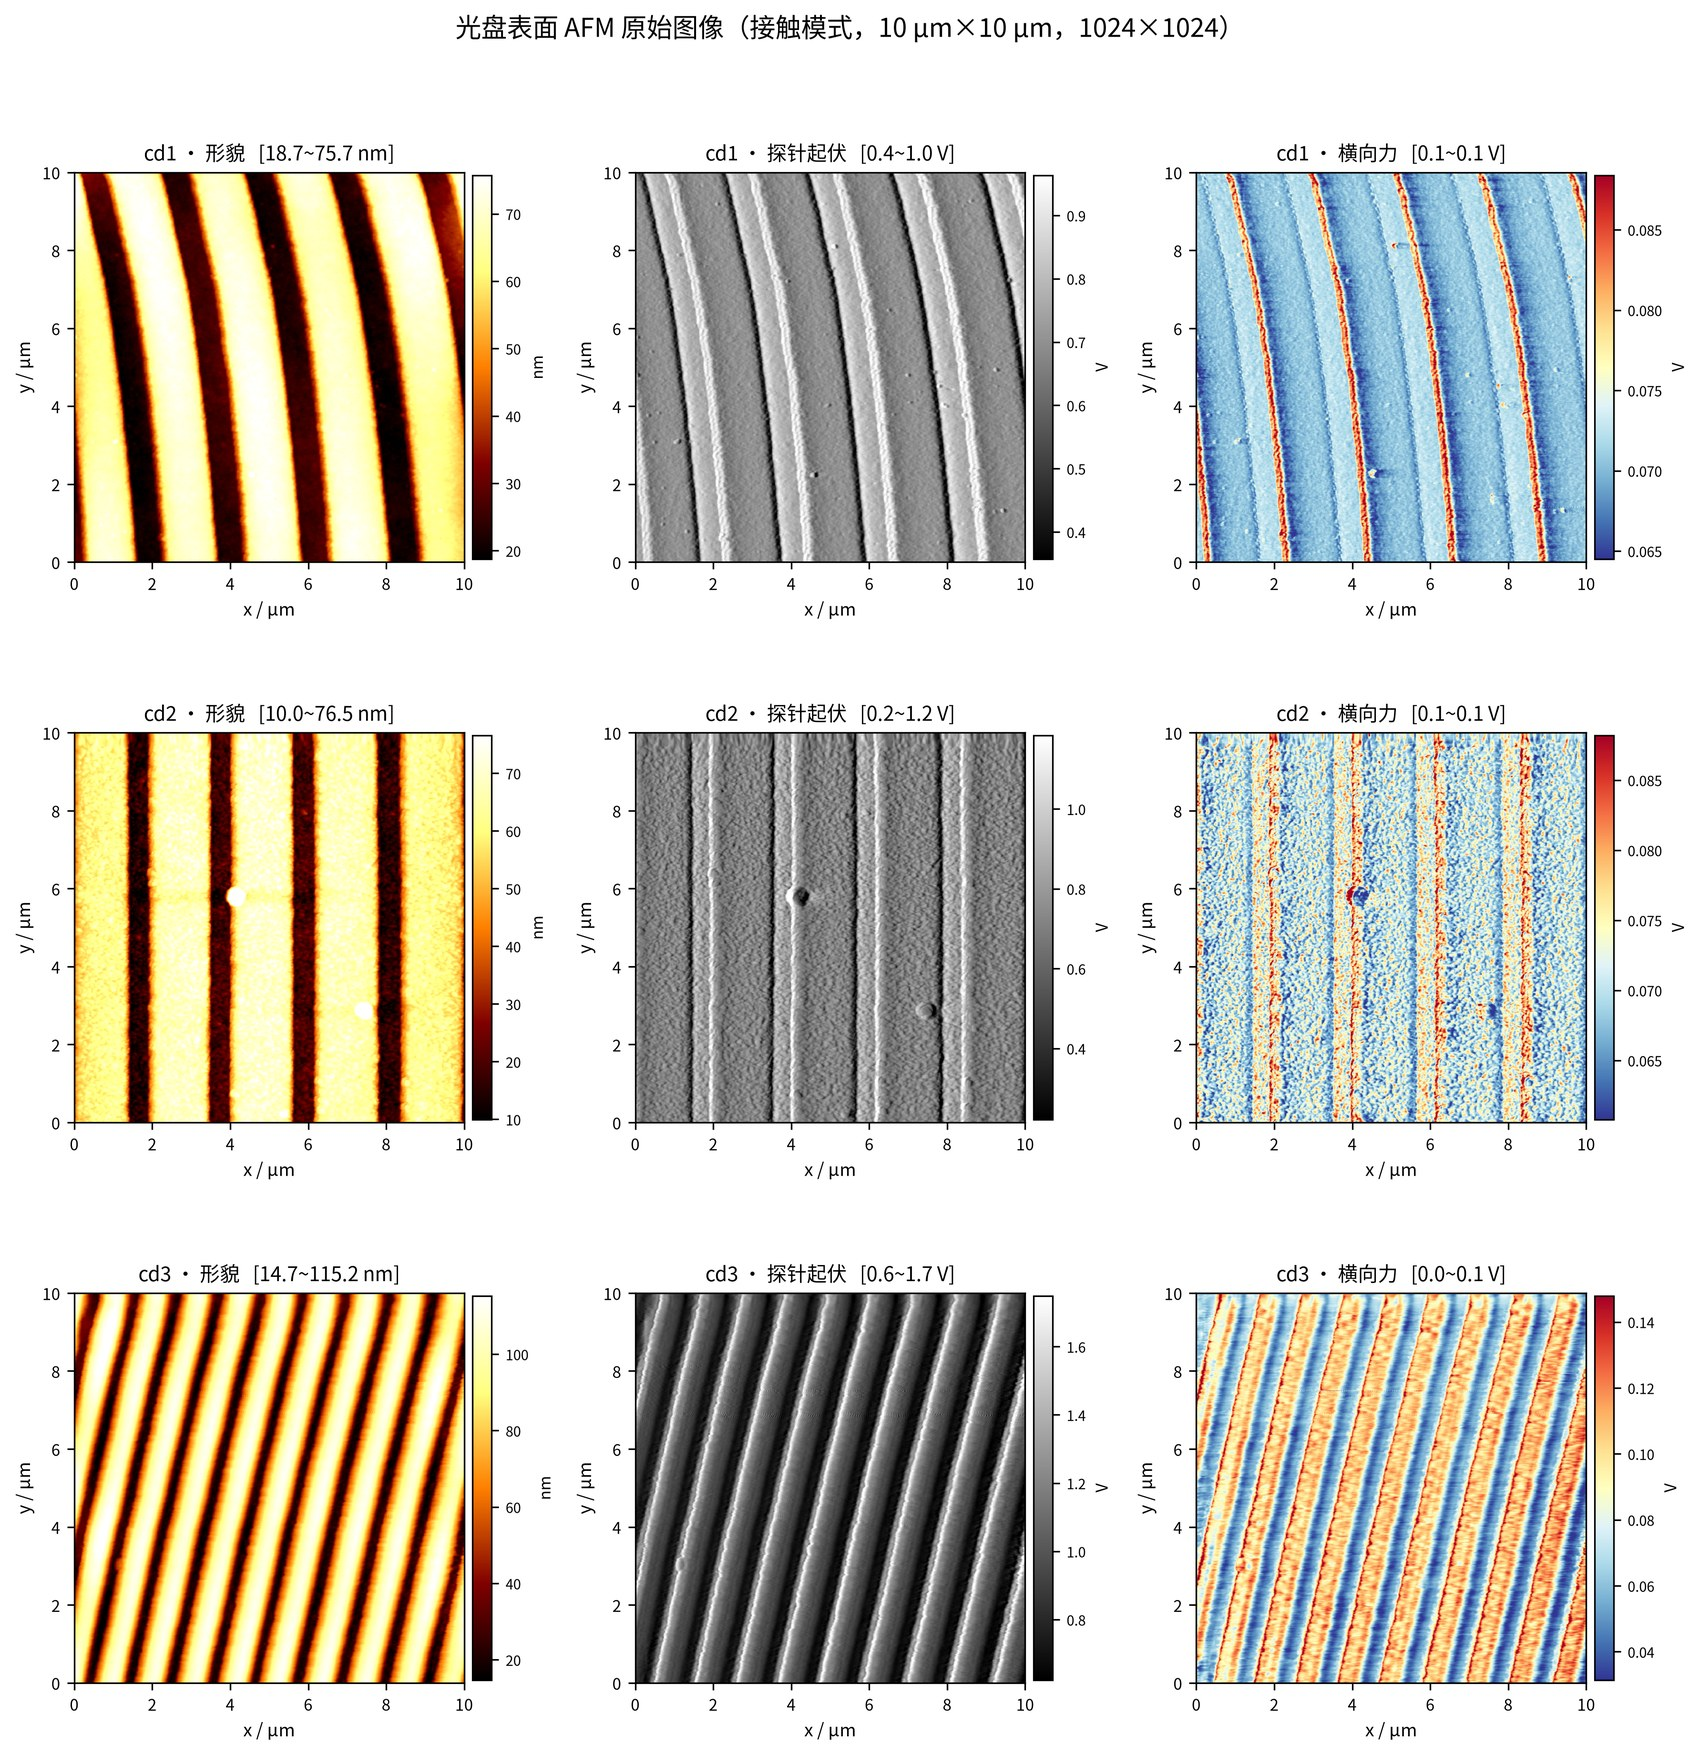
\includegraphics[width=0.95\textwidth]{fig01_overview_raw.jpg}
\caption{三张光盘的原始 AFM 图像（$10\,\mu\mathrm{m}\times10\,\mu\mathrm{m}$，$1024\times1024$ 点）。横向三列为形貌、误差信号（探针起伏）与横向力通道，纵向三行依次为 cd1、cd2、cd3。色标范围取各通道的第 0.5 与 99.5 百分位。}
\label{fig:overview}
\end{figure}

误差信号与横向力通道的图像对比度低于形貌通道，条纹结构仍可分辨，说明三路信号记录的是同一几何结构在不同物理量上的响应。三维形貌（图~\ref{fig:3d}）显示：三张光盘的表面都由“脊—槽”交替构成，脊顶平缓、槽底较窄，与光盘基片上宽岸窄槽的压制结构相符。

\begin{figure}[H]
\centering
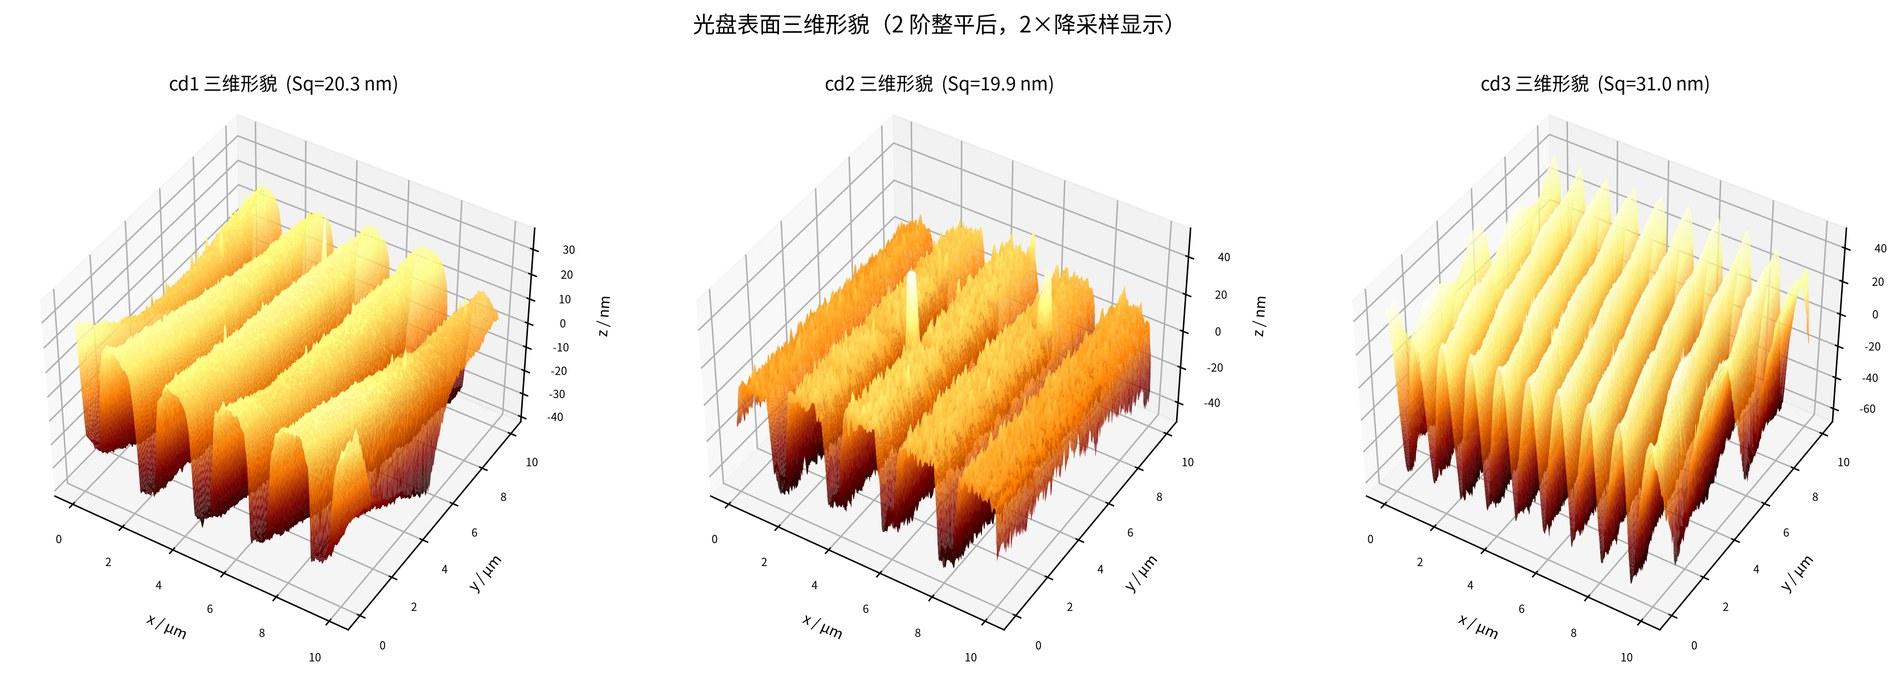
\includegraphics[width=0.95\textwidth]{fig02_3d_surface.jpg}
\caption{三张光盘的三维形貌（二阶面整平后，显示时作二倍降采样）。纵轴为高度，单位 nm。}
\label{fig:3d}
\end{figure}

\subsection{处理链的作用与面粗糙度参数}
\label{sec:rough}

面粗糙度按 Imager 手册 §47.2 的参数定义计算，八项参数的定义与物理含义列于附录~\ref{app:sparam}，全部在二阶面整平后的高度场上取；手册称其参数「基于二维标准并扩展到三维」，但未指明标准编号，其形式与 ISO 4287（二维轮廓）到 ISO 25178（面域）的对应关系一致；其中 $S_z$ 为十点高度，与 ISO 25178 的最大高度 $S_p+S_v$ 不同。

以 cd1 为例的处理链见图~\ref{fig:proc}。原始图像中沿 $x$ 方向的整体倾斜与弯曲由两阶处理扣除：逐行一阶拟合扣除了每行自身的倾斜与偏置，二阶面拟合扣除了跨行的慢变面形。处理后的行均值标准差为 0.03~nm（相对 $S_q$ 为 $1.5\times10^{-3}$），逐行偏置与扫描线台阶均已扣除；沿 $x$ 方向的列均值绝对电平（52.8~nm）整平后归零，而其起伏（标准差 8.45~nm）保持不变，说明二阶面整平只扣除了慢变面形，没有削弱条纹结构。

\begin{figure}[H]
\centering
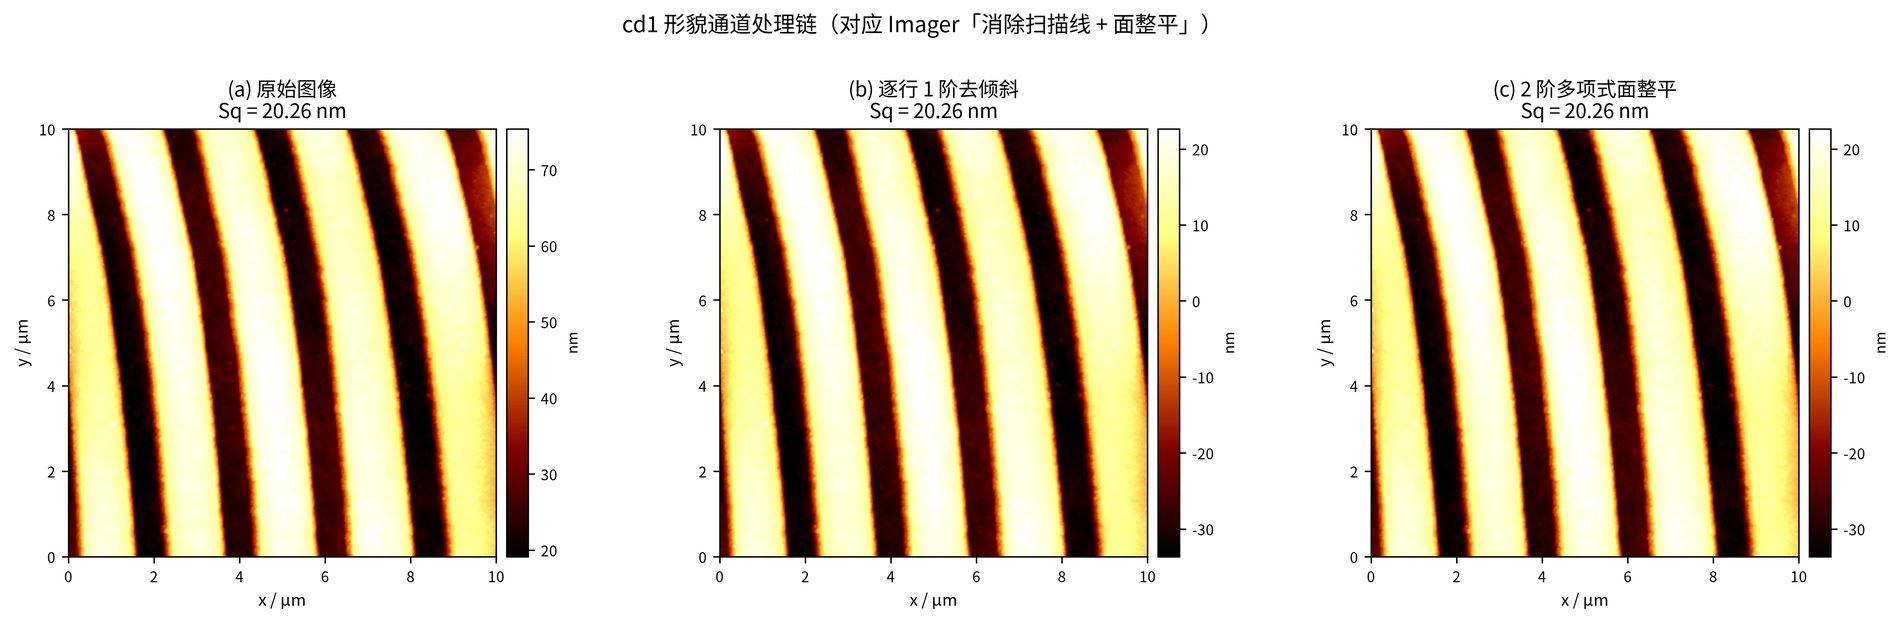
\includegraphics[width=0.95\textwidth]{fig03_processing_chain.jpg}
\caption{cd1 形貌通道的处理链：(a) 原始图像；(b) 逐行一阶多项式去倾斜；(c) 二阶面整平。三幅图的 $S_q$ 均为 20.26~nm。}
\label{fig:proc}
\end{figure}

处理前后的 $S_q$ 几乎不变（20.26~nm），这一结果的物理含义是：三张光盘的表面方差由条纹结构主导，扫描面与被测面之间的整体倾斜与弯曲贡献不足 0.1\%。与此对照，沿 $x$ 方向的列均值在三张光盘上的标准差分别为 8.45、19.60 与 2.20~nm，三者差异并不对应该方向的结构幅度，而与条纹倾角有关：倾斜越大，跨行平均对条纹的抵消越强，见第~\ref{sec:groove} 节。

面粗糙度参数列于表~\ref{tab:rough}。三张光盘的幅度参数随周期缩短而增大。三盘的偏度均为负值，说明高度分布相对中值偏向低处，即槽的面积占比小于脊，与表~\ref{tab:groove} 中占宽比大于 0.5 的结果一致；峭度均小于高斯分布的 3，说明高度分布比正态更平坦，反映脊顶与槽底各有一段近水平的平台，而不是单一峰值的随机起伏。均方根斜率 $S_{dq}$ 随周期缩短而增大、峰密度 $S_{ds}$ 则相反，二者分别对应更陡的槽壁与单位面积内更密的脊条。

\begin{table}[H]
\centering
\caption{三张光盘的面粗糙度参数（二阶面整平后，按 Imager 手册 §47.2 的定义计算；其中 $S_z$ 为十点高度）}
\label{tab:rough}
\small
\setstretch{1.0}
\begin{tabular}{@{}lcccccccc@{}}
\toprule
样品 & $S_a$/nm & $S_q$/nm & $S_y$/nm & $S_z$/nm & $S_{sk}$ & $S_{ku}$ & $S_{dq}$ & $S_{ds}/\mu\mathrm{m}^{-2}$ \\
\midrule
cd1 & 18.50 & 20.26 & 77.9 & 66.5 & $-0.54$ & 1.59 & 0.097 & 89.1 \\
cd2 & 16.61 & 19.94 & 102.4 & 94.5 & $-0.98$ & 2.49 & 0.153 & 72.2 \\
cd3 & 26.95 & 31.02 & 115.9 & 113.5 & $-0.49$ & 1.89 & 0.223 & 40.8 \\
\bottomrule
\end{tabular}
\end{table}

\subsection{沟槽周期与峰谷深度}
\label{sec:groove}

周期由逐行一维傅里叶变换的主峰给出，取 1024 行的中位数，四分位区间作为行间散布的度量。结果列于表~\ref{tab:groove}：cd1 与 cd2 的周期分别为 2170 与 2143~nm，行间四分位区间宽度不超过 15~nm；cd3 的周期为 1090~nm，行间散布仅 3~nm。该散布说明三张光盘的沟槽在视场内的周期均匀，逐行测量的重复性满足定量比较的需要。

\begin{table}[H]
\centering
\caption{沟槽几何参数（长度单位 nm，倾角单位 $^\circ$）}
\label{tab:groove}
\small
\setstretch{1.0}
\begin{tabular}{@{}lcccccc@{}}
\toprule
样品 & 周期$^\ast$ & 行间四分位区间 & 倾角 & 峰值深度$^\dagger$ & 占宽比 & 修正周期 \\
\midrule
cd1 & 2170 & 2167--2175 & $+8.1$ & 55.2 & 0.61 & 2149 \\
cd2 & 2143 & 2137--2151 & $+0.0$ & 60.4 & 0.75 & 2143 \\
cd3 & 1090 & 1089--1092 & $-13.2$ & 93.4 & 0.63 & 1062 \\
\bottomrule
\end{tabular}

\vspace{2pt}
\footnotesize $^\ast$ 逐行一维傅里叶变换主峰的行中位数；$^\dagger$ 逐行 15 点（约 146~nm）平滑剖面的 $P_{99}-P_1$ 的 1024 行中位数；修正周期为按倾角余弦修正后的值；倾角为条纹与慢扫方向（$y$ 轴）的夹角，正值表示条纹随行号向 $+x$ 漂移。
\end{table}

条纹倾角由式~\eqref{eq:tilt} 给出，cd1 为 $+8.1^\circ$、cd3 为 $-13.2^\circ$、cd2 接近 $0^\circ$。相位漂移中各成分的定量分解见表~\ref{tab:drift}。cd3 的漂移几乎全部落在一次项上：二次项与三次项合计不足总量的 2.2\%，一次拟合的残差为 0.013 个周期，说明它是恒定的横向位移，即条纹与扫描轴之间的固定夹角；cd2 的总漂移只有 0.01 个周期，没有系统性位移。cd1 的漂移同样以一次项为主，二次与三次项相对弦线的单侧偏离分别为 0.115 与 0.050 个周期（占漂移总量的 16.5\% 与 7.2\%，与表~\ref{tab:drift} 同口径），一次拟合的残差为 0.035 个周期；把视场按 $y$ 分为 8 个 128 行的分带后，局部条纹方向相对慢扫轴由 $15.4^\circ$ 单调降到 $4.4^\circ$，变化量 $11.0^\circ$；用结构张量分块法独立核验，条纹法线角由 $-14.9^\circ$ 转到 $-4.0^\circ$，变化量 $10.8^\circ$，与相位法的结果一致。该变化等效的曲率半径为 $L/\Delta\theta\approx53\,\mu\mathrm{m}$，只有盘片数据区半径（25--58~mm）的 $1/1100$--$1/470$，且同一批次的 cd2 与 cd3 都没有这一现象，故不能归因于盘片的轨道曲率，其量级与压电执行器的蠕变、迟滞一类的逐次效应相符\cite{croft2001}。

沿 $x$ 方向的相位场同样存在可测的二次项。用二维傅里叶带通解调（中心取主场频 $f_0$，高斯半宽 $1.2\times10^{-3}$ 与 $8\times10^{-3}$ 周期/像素）直接读出相位场，再对归一化横坐标 $v$ 作最小二乘，三张样品的 $v^2$ 系数为 $-0.12$、$-0.18$ 与 $-0.35$ 个周期，对应视场边缘 62--98~nm 的横向位移，折成等效曲率半径为 0.13--0.20~mm；另写的一套滑窗解调给出 0.07--0.11~mm，两种独立方法的量级一致。该半径比盘片数据区半径（25--58~mm）小两个数量级，且三张样品取同一量级而它们分属两种规格，故判为仪器侧效应，即扫描器 $x$ 轴标尺的非均匀或扫描头的弓形轨迹，不是盘片几何。把已知的二次位移场注入图像后重复整条处理流程，$v^2$ 系数按注入量线性恢复（边缘矢高 0.5、2、8~nm 对应 $-9.1\times10^{-4}$、$-3.6\times10^{-3}$、$-1.5\times10^{-2}$ 个周期），说明该估计对曲率确有响应；由拟合残差给出的 2$\sigma$ 检出限对应 0.3--3.3~nm 的矢高。盘片轨道在 $10\,\mu\mathrm{m}$ 视场内的矢高只有 0.2--0.5~nm（按各自周期折算为 $1\times10^{-4}$--$5\times10^{-4}$ 个周期），比实测的 62--98~nm 小两个数量级，也处在检出限的边缘或以下，因此轨道曲率既不是相位漂移的主因，也无法从本数据中分离出来。条纹方向随 $x$ 的剪切为 $0.2^\circ$--$0.5^\circ$，cd2 与 cd1、cd3 同量级而其漂移几乎为零，同样不作物理归因。

\begin{table}[H]
\centering
\caption{条纹相位漂移的多因素分解（相位单位：周期）}
\label{tab:drift}
\footnotesize
\setstretch{1.0}
\begin{tabular}{@{}lcccccc@{}}
\toprule
样品 & 倾角 & 漂移总量 & 线性项 & 二次垂度 & 三次端项 & 一次拟合残差 \\
\midrule
cd1 & $+8.1^\circ$ & $-0.70$ & $-0.60$ & $0.115$（16.5\%） & $-0.050$（7.2\%） & 0.035 \\
cd2 & $+0.0^\circ$ & $0.01$ & $-0.02$ & 0.009 & 0.011 & 0.007 \\
cd3 & $-13.2^\circ$ & $2.15$ & $2.15$ & $-0.040$（1.9\%） & $-0.002$（0.1\%） & 0.013 \\
\bottomrule
\end{tabular}

\vspace{2pt}
\footnotesize 漂移总量为全场相位差；线性项为一次项在全视场（1024 行）内的累计变化量（其除以行数即逐行斜率）；二次垂度为二次项相对弦线的最大偏离，括号内为其占漂移总量的比例；三次端项为三次项在视场端点处相对弦线的附加量（取半幅，与二次垂度同为单侧量）；一次拟合残差为扣除线性项后的均方根。cd2 的漂移量本身接近零，其比例不具物理意义，故不给出。
\end{table}

倾角的直接后果体现在平均剖面上：若不做行程对齐，跨 1024 行平均时 cd3 的条纹相位漂移达 2.1 个周期（对应 2.3~$\mu$m 的横向位移），条纹在平均中相互抵消，平均剖面的峰谷（$P_{99}-P_1$）只剩 8.1~nm，为对齐后 88.6~nm 的 9.1\%（cd1 的同口径数值为 28.5 与 52.6~nm，低估 46\%；cd2 的倾角接近零，两者相同，为 56.1~nm）；对齐后再平均，峰谷恢复到 88.6~nm，与逐行统计的 93.4~nm 相差 5.2\%。本文比较了三种对齐方式：全局单斜率（本文采用）、逐行相位对齐，以及按拟合相位场逐行逐窗口的二维对齐。后两者相对全局单斜率的总量增益只有 0.4\%（cd3）与 0.1\%（cd1），cd2 因无漂移三者相差在 0.2\% 的噪声以内；非线性成分只占漂移两成、且表现为条纹方向的缓变而非整体错位，这与增益之小相符。因此本实验的沟槽深度与周期读数不受对齐方式选择的影响。图~\ref{fig:prof} 给出对齐后的平均剖面，cd2 的剖面呈现宽脊与窄槽的矩形轮廓，占宽比 0.75；cd1 与 cd3 的轮廓更接近对称，占宽比 0.61 与 0.63。按占宽比与周期折算，cd1--cd3 的脊宽分别为 1318、1614 与 688~nm，槽宽分别为 852、530 与 403~nm。

\begin{figure}[H]
\centering
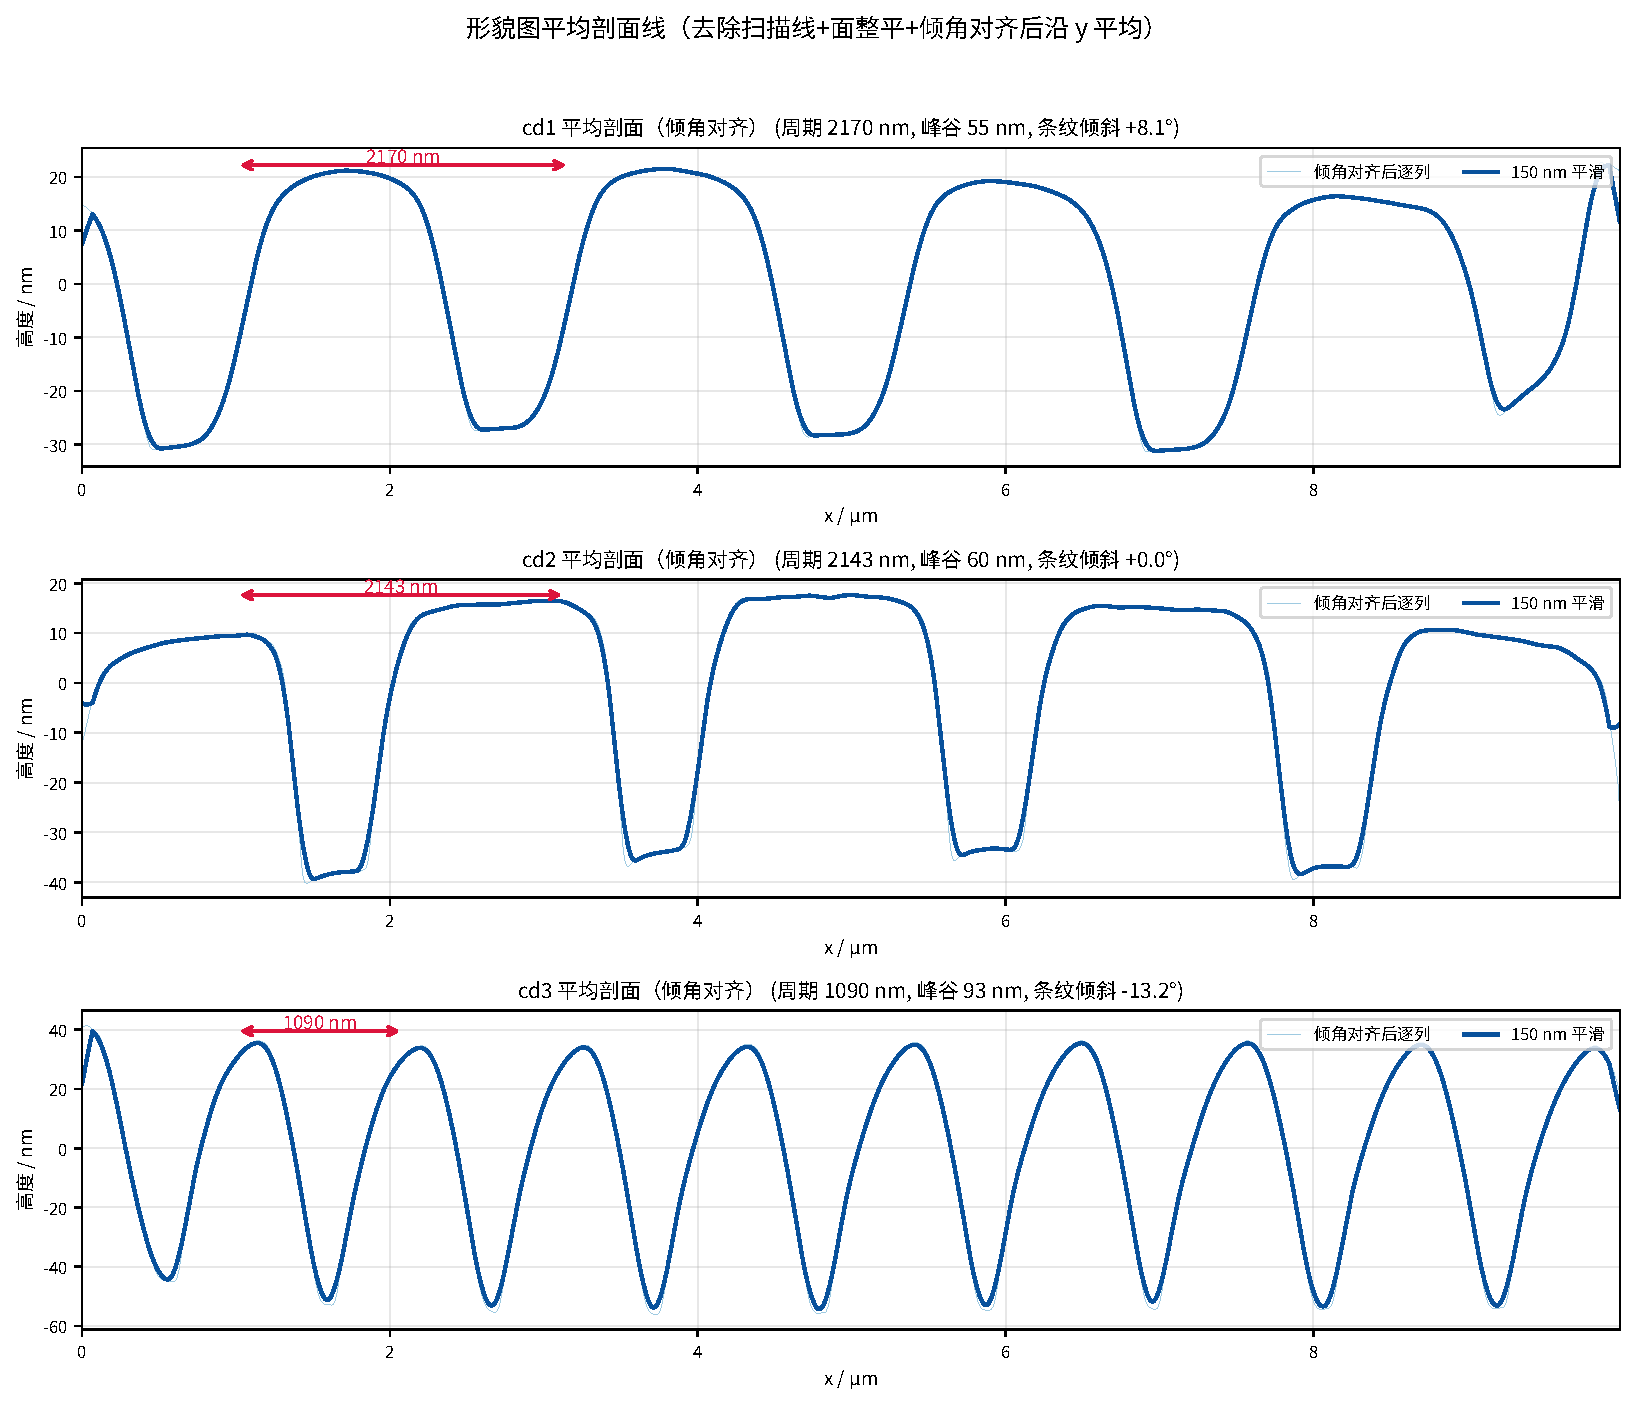
\includegraphics[width=0.95\textwidth]{fig04_profiles.pdf}
\caption{三张光盘的平均剖面（去扫描线、面整平、按条纹倾角对齐后沿 $y$ 平均）。细线为对齐后的逐列数据，粗线为 150~nm 平滑结果，箭头标注主周期。}
\label{fig:prof}
\end{figure}

峰谷深度在 55--93~nm 之间，随周期缩短而增大。这一读数并不等于沟槽的真实深度：探针以有限的曲率半径与锥角接近样品，槽壁对针尖的遮挡使针尖无法到达槽底，测得的槽型被展宽、深度被压缩。手册给出的量级估计为\cite{manual_cspm}：对台阶，若针尖半锥角为 $10^\circ$，单边展宽约为台阶高度的 18\%；对颗粒，展宽使粒径读数偏大约 20\% 并叠加 $2R$，$R$ 为针尖曲率半径。以此作为量级参照，本文的深度读数应视为下限，真实槽深大于表中数值。作为横向对照，文献用同类型仪器（CSPM-3100）测得 CD 的沟槽周期 1700~nm、深度 196~nm，DVD 的周期 900~nm、深度 218~nm\cite{sunzhi2006}；该文使用曲率半径 20~nm 的探针、$512\times512$ 采样、3~Hz 扫描频率。本文倾角修正后的周期比其偏大 26\% 与 18\%（按未修正的表观值为 28\% 与 21\%）；这一比较尚未扣除横向标定因子 $k$，绝对尺度的讨论见第~\ref{sec:calib} 节。周期偏大、深度偏小这一组合，与“横向尺度标定偏大、纵向受针尖卷积压缩”的判断方向一致。

\subsection{频谱特征}

平均剖面的一维功率谱与二维傅里叶谱见图~\ref{fig:spec}。一维谱的主峰波长与表~\ref{tab:groove} 的周期一致，并在 $1/2$、$1/3$ 基频处出现谐波。二次谐波与基频的幅度比为 cd1 18.7\%、cd2 43.5\%、cd3 20.1\%，说明 cd2 的轮廓最接近方波（与其占宽比 0.75 的矩形剖面一致），cd1 与 cd3 更接近正弦。cd3 的基频峰最窄（归一化半高宽 0.33，另两组均为 0.60），与其行间周期散布最小一致。

二维傅里叶谱的峰位给出条纹法线方向。受视场限制，$k$ 空间的采样间隔为 $0.1\,\mu\mathrm{m}^{-1}$，据此估计的方向角分辨率为数度，与相位斜率法相比低一个量级，故本文的倾角一律取相位斜率法的结果，二维谱只用于确认条纹的一维周期性（能量集中在 $k_x$ 轴上）。

\begin{figure}[H]
\centering
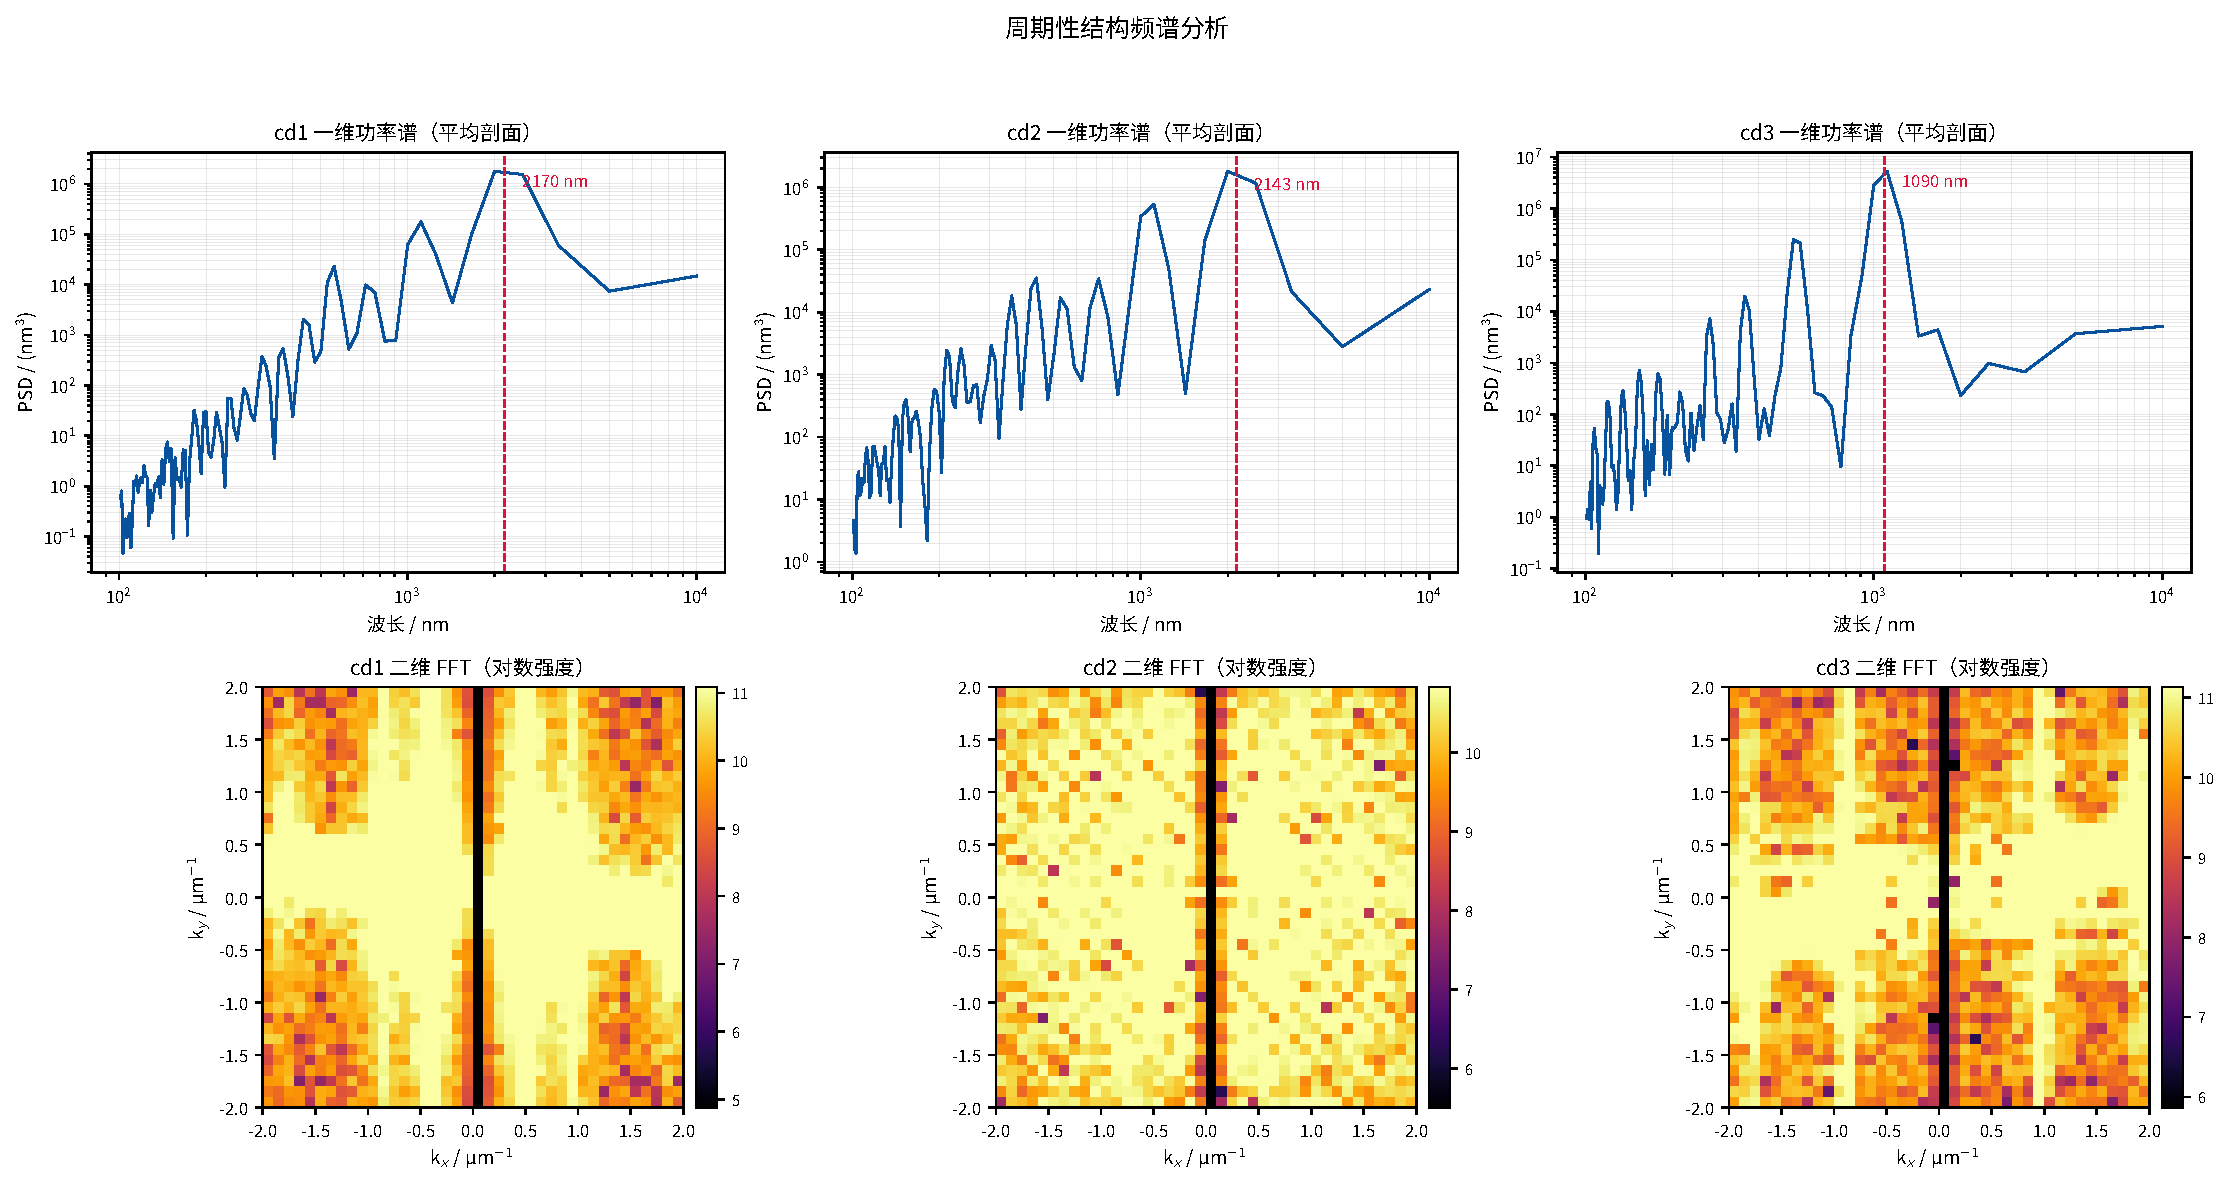
\includegraphics[width=0.95\textwidth]{fig05_spectra.pdf}
\caption{上排：平均剖面的一维功率谱密度（对数坐标，虚线为主周期）；下排：整平后形貌的二维傅里叶谱（对数强度，显示范围 $\pm2\,\mu\mathrm{m}^{-1}$）。}
\label{fig:spec}
\end{figure}

\subsection{横向尺度标定与光盘类型的推断}
\label{sec:calib}

三张光盘的表观周期为 2170、2143 与 1090~nm，与 CD（1600~nm）、DVD（740~nm）的标称道距均不相同：cd1 与 cd2 的周期接近，cd3 的周期约为二者的二分之一，三张盘不构成同一种格式的一组测量。扫描器的横向标定与样品道距本身的差别，都会使表观周期偏离标称道距。

cd1 与 cd2 的周期在倾角修正后为 2149 与 2143~nm，相对差 0.25\%。两者的测量条件相同（同一扫描器、同一视场、同一扫描频率），行间偏差不足以解释这一量级的差异，故在本数据的精度内可视为同一规格；该判断只涉及两盘道距的一致性，不涉及二者的绝对尺度。

以 CD 道距 1600~nm 为参照时，$k=2146/1600=1.34$，同一因子把 cd3 的周期修正为 $1062/1.34=792$~nm，与 DVD 道距 740~nm 相差 $+7.0\%$；反向以 DVD 道距 740~nm 为参照时，$k=1062/740=1.44$，同样把 cd1 与 cd2 修正为 1496~nm，比 CD 道距低 6.5\%。两种参照下的残余差异同为 7\% 量级，与探针在沟槽边缘的卷积、扫描器非线性以及盘片道距公差相当，故在本数据的精度内，数据支持的组合为 cd1、cd2 属 CD 类、cd3 属 DVD 类，快扫轴的横向标定偏大 1.34--1.44 倍。

逐盘比值由手算给出，未计入观测噪声与倾角的不确定度，也无法给出标定因子的区间。为把上述判断写成带不确定度的估计，本文以 ECMA 标准道距为约束，对三张光盘的周期作贝叶斯联合拟合。生成模型取
\begin{equation}
P_{\text{obs},i}=\frac{k\,p_i}{\cos\alpha_i},
\label{eq:scale}
\end{equation}
其中 $P_{\text{obs},i}$ 为第 $i$ 张盘的表观周期（逐行一维傅里叶变换主峰的行中位数，见表~\ref{tab:groove}）；$k$ 为横向标定因子，即观测量与真值之比（$k>1$ 表示标称 $10\,\mu\mathrm{m}$ 视场对应的真实行程小于 $10\,\mu\mathrm{m}$）；$p_i$ 为标准道距；$1/\cos\alpha_i$ 为条纹倾角对沿快扫轴截距的放大。待比较的五个模型、先验与采样设定见表~\ref{tab:models}。

逐盘后验的标定因子与等效伸缩系数列于表~\ref{tab:scale} 的中段与末行。三者的后验中位数与“倾角余弦修正后除以标称道距”的精确解（1.3429、1.3395 与 1.4346）相对偏差均小于 0.15\%，说明采样已收敛到解析最优点；这一比较不构成对模型的检验。折算成伸缩系数，前两张光盘比铭牌值低 25\%，cd3 低 30\%。

\begin{table}[H]
\centering
\caption{表观周期过冲的因素分解（相对格式标准的标称道距）}
\label{tab:scale}
\footnotesize
\setstretch{1.0}
\begin{tabular}{@{}lccc@{}}
\toprule
项目 & cd1 & cd2 & cd3 \\
\midrule
表观周期 $P_{\text{obs}}$ / nm & 2170.45 & 2143.26 & 1090.40 \\
标称道距 $p$ / nm & 1600 & 1600 & 740 \\
表观过冲 & $+35.7\%$ & $+34.0\%$ & $+47.4\%$ \\
\midrule
横轴标定 $k$（后验）& $1.341\pm0.018$ & $1.338\pm0.018$ & $1.433\pm0.020$ \\
\quad 精确解（不含噪声）& 1.3429 & 1.3395 & 1.4346 \\
\quad 占过冲的比例 & 96\% & 100\% & 91\% \\
倾角投影 $1/\cos\alpha-1$ & $+1.0\%$ & $0.0\%$ & $+2.7\%$ \\
针尖卷积 & $0\%$ & $0\%$ & $0\%$ \\
拟合残余 & $+0.1\%$ & $+0.1\%$ & $+0.1\%$ \\
\midrule
等效伸缩系数 / (nm\,V$^{-1}$) & 187.2 & 187.5 & 175.2 \\
\bottomrule
\end{tabular}

\vspace{2pt}
\footnotesize 说明：各因素的百分比是乘性分解的线性近似，横轴标定、倾角投影、针尖卷积与拟合残余四项相加与表观过冲不完全相等。“占过冲的比例”为 $(k-1)$ 与表观过冲之比。拟合残余为上述四项之和对表观过冲的残差，反映后验中位数相对精确解的 0.1\% 差异。表中 $k$ 的后验区间只计入 1\% 的周期测量噪声；标准道距的公差（CD $\pm6.25\%$、DVD $\pm4.05\%$）属不确定度项而非偏差项，若一并计入，$k$ 的不确定度将增大到 $\pm6\%$ 量级。
\end{table}

模型比较的结果见表~\ref{tab:models}。在“盘为标称 CD/DVD”的前提下，cd1、cd2 为 CD 而 cd3 为 DVD 的假设残差为 $-2.0\%$、$-2.2\%$ 与 $+4.5\%$；“全 CD”与“全 DVD”的残差都达 33\%，二者在道距固定、$k$ 自由时只依赖乘积 $kp$，数学上是同一个模型，因此它们的失败与“CD 还是 DVD”的取舍无关，只说明三盘不能用单一比例描述。$k=1$、三道距自由的模型残差小于 0.2\%、似然更高，但那是以三个自由尺度拟合三个数据点的必然结果，且给出的道距（2149、2143 与 1062~nm）不对应任何已知格式。似然差的绝对值随噪声设定而变，故这里的比较只用残差，不以其作为证据强度。

\begin{table}[H]
\centering
\caption{联合拟合的模型设定、先验与比较结果}
\label{tab:models}
\footnotesize
\setstretch{1.0}
\begin{tabularx}{\textwidth}{@{}l X c c c@{}}
\toprule
模型 & 道距设定 & 自由参数 & $\ln L$ & 残差 \\
\midrule
H1 & cd1、cd2 取 CD（1600~nm），cd3 取 DVD（740~nm）；三盘共享 $k$ & 4 & $-25.7$ & $-2.0/-2.2/+4.5\%$ \\
H2 & 三盘均取 CD（1600~nm）；共享 $k$ & 4 & $\approx-1.7\times10^{3}$ & 33\% \\
H3 & 三盘均取 DVD（740~nm）；共享 $k$ & 4 & $\approx-1.7\times10^{3}$ & 33\% \\
H4 & 道距同 H1；三盘各自独立取 $k$ & 6 & $-11.3$ & $<0.2\%$ \\
H5 & $k=1$，三道距自由 & 6 & $-11.3$ & $<0.2\%$ \\
\bottomrule
\end{tabularx}

\vspace{2pt}
\footnotesize 说明：$\ln L$ 取 $\sigma=1\%$ 的周期方法误差、$\alpha_i$ 固定于实测值。先验与采样设定为：$\log k\sim N(0,\,0.35^{2})$，其 $\pm2\sigma$ 对应因子区间 0.50--2.0，不作强约束；$\alpha_i$ 取以相位斜率法实测值为中心、宽度 $0.3^\circ$ 的正态先验；采样用自写的仿射不变系综采样器（affine-invariant ensemble sampler，20 个 walker），每个模型取 $1.8\times10^{5}$--$2.1\times10^{5}$ 个后验样本，自相关时间 17--26，有效样本数 $6.8\times10^{3}$--$1.0\times10^{4}$。H2 与 H3、H4 与 H5 分别只差参数的换元，似然完全相同；$\ln L$ 的绝对值随 $\sigma$ 假设而变（$\sigma$ 取 2\% 与 5\% 时，H1 与 H2 的差分别为 425 与 68），故不宜用作证据强度。
\end{table}



针尖卷积不改变周期读数：周期 740--2170~nm 与针尖横向尺寸（顶点半径约 10--20~nm、半锥角 $10^\circ$，对应的横向尺度在数十 nm 以内）之比大于 18，而一阶卷积只展宽凸起、压窄压浅凹陷，不改变同类特征之间的间距。

迟滞、蠕变与压电非线性会使周期随位置变化。本数据中这类效应确有痕迹，但幅度很小：按慢扫方向把视场分成 8 个 128 行的条带，各带周期中位数的极差为 0.6\%、0.9\% 与 0.4\%，折合 13、20 与 5~nm；逐行周期随行号的线性斜率为 $-0.014$、$+0.017$ 与 $+0.004$~nm/行，折合整幅 $-14$、$+17$ 与 $+4$~nm。cd1 与 cd2 的斜率反号，说明它不是单向的蠕变。即使把这 0.8\% 全部计入标定误差，也只占 34\%--47\% 表观过冲的百分之二，因此位置相关项不是主因；但它是真实存在的，应计入 $k$ 的系统误差预算。

另一种解释是把沟槽与岸的成对结构判读为半周期或二次谐波，即 cd3 的真实周期是 cd1、cd2 的一半。这一解释与剖面数据不符：cd3 的平均剖面在一个 1062~nm 周期内只出现一次完整的脊—槽循环，相邻谷的间距逐段实测为 1035、1064、1055、1074、1084、1084、1113 与 1123~nm，八个间隔都接近同名周期，不存在 $2\times1062$~nm 的包络调制；cd1 的相邻谷间距实测为 2090、2158、2207 与 2266~nm，未见 1075~nm 量级的亚结构（cd2 的宽脊平台上存在次极值，逐段间距不稳，不作此判据）。因此 cd3 与两张 CD 的周期比 2:1 不来自半周期或二次谐波的误判；该比值反映样品之间的周期差异，其绝对尺度仍受 $k$ 与 $p$ 不可分离的限制。

\textbf{$k$ 与道距在本数据中不可分离。}式~\eqref{eq:scale} 中 $k$ 与 $p_i$ 只以乘积出现，两者同时自由时后验相关系数为 $-0.999$，数据本身不能把二者分开；$k=1.34$ 是以“盘片道距等于标称值”为前提的条件结论，不是独立测得的标定值。

该前提取不同值时给出不同图景。按仪器标称尺度换算（$k=1$）时，三盘道距由表~\ref{tab:groove} 的修正周期给出，为 2149、2143 与 1062~nm，不对应任何已知光盘格式；取 $k=1.34$ 时，三盘道距为 1600、1600 与 792~nm，前两者正是 CD 的标准道距。

cd3 的标定因子比两张 CD 高 6.9\%，有两种自洽的解释。其一是三次采集各自独立完成：每次测量前取下前一样品、重新装样并把仪器调整回测量状态，cd3 的信号增益（5.0）与满量程高度（147.39~nm）也与前两次不同，三次之间的横向标定状态未必等同；其二是 cd3 本身为道距 0.8~$\mu$m 量级的盘片。本数据无法区分这两种解释。

同厂另一型号仪器的实测偏差方向与本数据一致，量级则小得多。孙志等在本原 CSPM-3100 上测得 CD-R 的道距为 1700~nm、DVD-R 为 900~nm\cite{sunzhi2006}；按 ECMA-130 与 ECMA-267 规定的标称道距 1.6~$\mu$m 与 0.74~$\mu$m\cite{ecma130,ecma267} 计，二者分别偏大 6.25\% 与 21.6\%（比值 3.46），其中 DVD 的偏差约为 CD 的 3.5 倍，与本数据中 cd3 的标定因子高于 cd1、cd2 的方向一致。该文所用仪器型号与探针均与本机不同，偏差量级也只有本数据的约 $1/5$ 与 $1/2$，故此处只取偏差方向作为佐证，不以该文数值校核本文的 $k$。

仪器手册在四个标称周期 3000~nm 光栅的校正算例中，给出四个扫描方向的实测周期 2489--3533~nm，相对偏差 $-17.0\%$ 至 $+17.8\%$\cite{manual_cspm}。该算例说明同一台仪器不同扫描方向的横向标定可相差 10\% 以上，量级上支持把 34\%--47\% 的表观过冲归因于扫描器标定一侧。

上述标定因子不是独立测量的结果：本实验未用标准光栅校正扫描器的横向标尺，三张盘片的型号亦未记录，$k$ 的数值以 CD 与 DVD 的标称道距为参照反推得到，其成立依赖“盘片道距等于标称值”这一前提。若需与本数据无关的独立标定值，应按手册 §17.1 的流程\cite{manual_cspm} 用已知周期的标准光栅重作校正，或补记盘片的实际型号。

横向标定不进入高度参数的换算：$z$ 由文件头记录的满量程高度单独换算，与 $x$、$y$ 的伸缩系数无关。但 $S_{dq}$ 与 $S_{ds}$ 依赖横向像素尺度（前者按像素间距取梯度，后者以评定面面积为分母），表~\ref{tab:rough} 中的这两项按名义像素尺度 9.77~nm 计算，若 $k$ 被修正，二者应按同一比例换算。

\subsection{误差信号与横向力通道}

三路信号的统计量列于表~\ref{tab:signal}。误差信号的标准差折合满量程的 7.6\%--13.8\%，横向力的相应值为 2.7\%--16.9\%，两者都以 cd3 最大。

\begin{table}[H]
\centering
\caption{误差信号与横向力通道的统计量（已扣除逐行偏置）}
\label{tab:signal}
\small
\setstretch{1.0}
\begin{tabular}{@{}llcccc@{}}
\toprule
样品 & 通道 & 满量程 & 标准差 & 峰谷值 & 相对满量程 \\
\midrule
\multirow{2}{*}{cd1} & 误差信号 & 1.429~V & 0.1088~V & 0.943~V & 7.6\% \\
                     & 横向力   & 0.143~V & 0.0039~V & 0.045~V & 2.7\% \\
\multirow{2}{*}{cd2} & 误差信号 & 1.429~V & 0.1478~V & 1.398~V & 10.3\% \\
                     & 横向力   & 0.143~V & 0.0051~V & 0.068~V & 3.6\% \\
\multirow{2}{*}{cd3} & 误差信号 & 2.000~V & 0.2750~V & 1.524~V & 13.8\% \\
                     & 横向力   & 0.167~V & 0.0282~V & 0.154~V & 16.9\% \\
\bottomrule
\end{tabular}
\end{table}

误差信号正比于形貌沿扫描方向的变化率，因而在槽壁处最大、在平台处趋于零。图~\ref{fig:chan} 给出三路信号的单行剖面：形貌通道给出“脊—槽”的绝对高度，误差信号在高度转折处出现尖峰，横向力在槽壁两侧出现符号相反的偏转。针尖上坡与下坡时悬臂的扭转变形方向相反，横向力信号因此在每一周期的两侧呈反对称，这是摩擦力的特征。三张光盘中 cd3 的横向力相对幅度最大（16.9\%），与其结构最深（93.4~nm）和周期最短（1090~nm）一致：在相同的法向载荷下，更陡的槽壁产生更大的扭转。

三路信号在个别像素上达到了 16 位满量程（原始量 65535）：cd2 形貌 27 个像素、cd3 横向力 35 个像素，两路误差信号另有 4 与 6 个像素。达到满量程意味着真实信号超出该通道的显示范围，因此表~\ref{tab:rough} 中 cd2 的 $S_y$（102.4~nm，已贴近满量程 105.28~nm）与表~\ref{tab:signal} 中 cd3 横向力的峰谷值（0.154~V，为满量程的 92\%）应视为下限；削顶像素占比低于 $10^{-4}$，对标准差的影响可忽略，周期读数不受影响。

\begin{figure}[H]
\centering
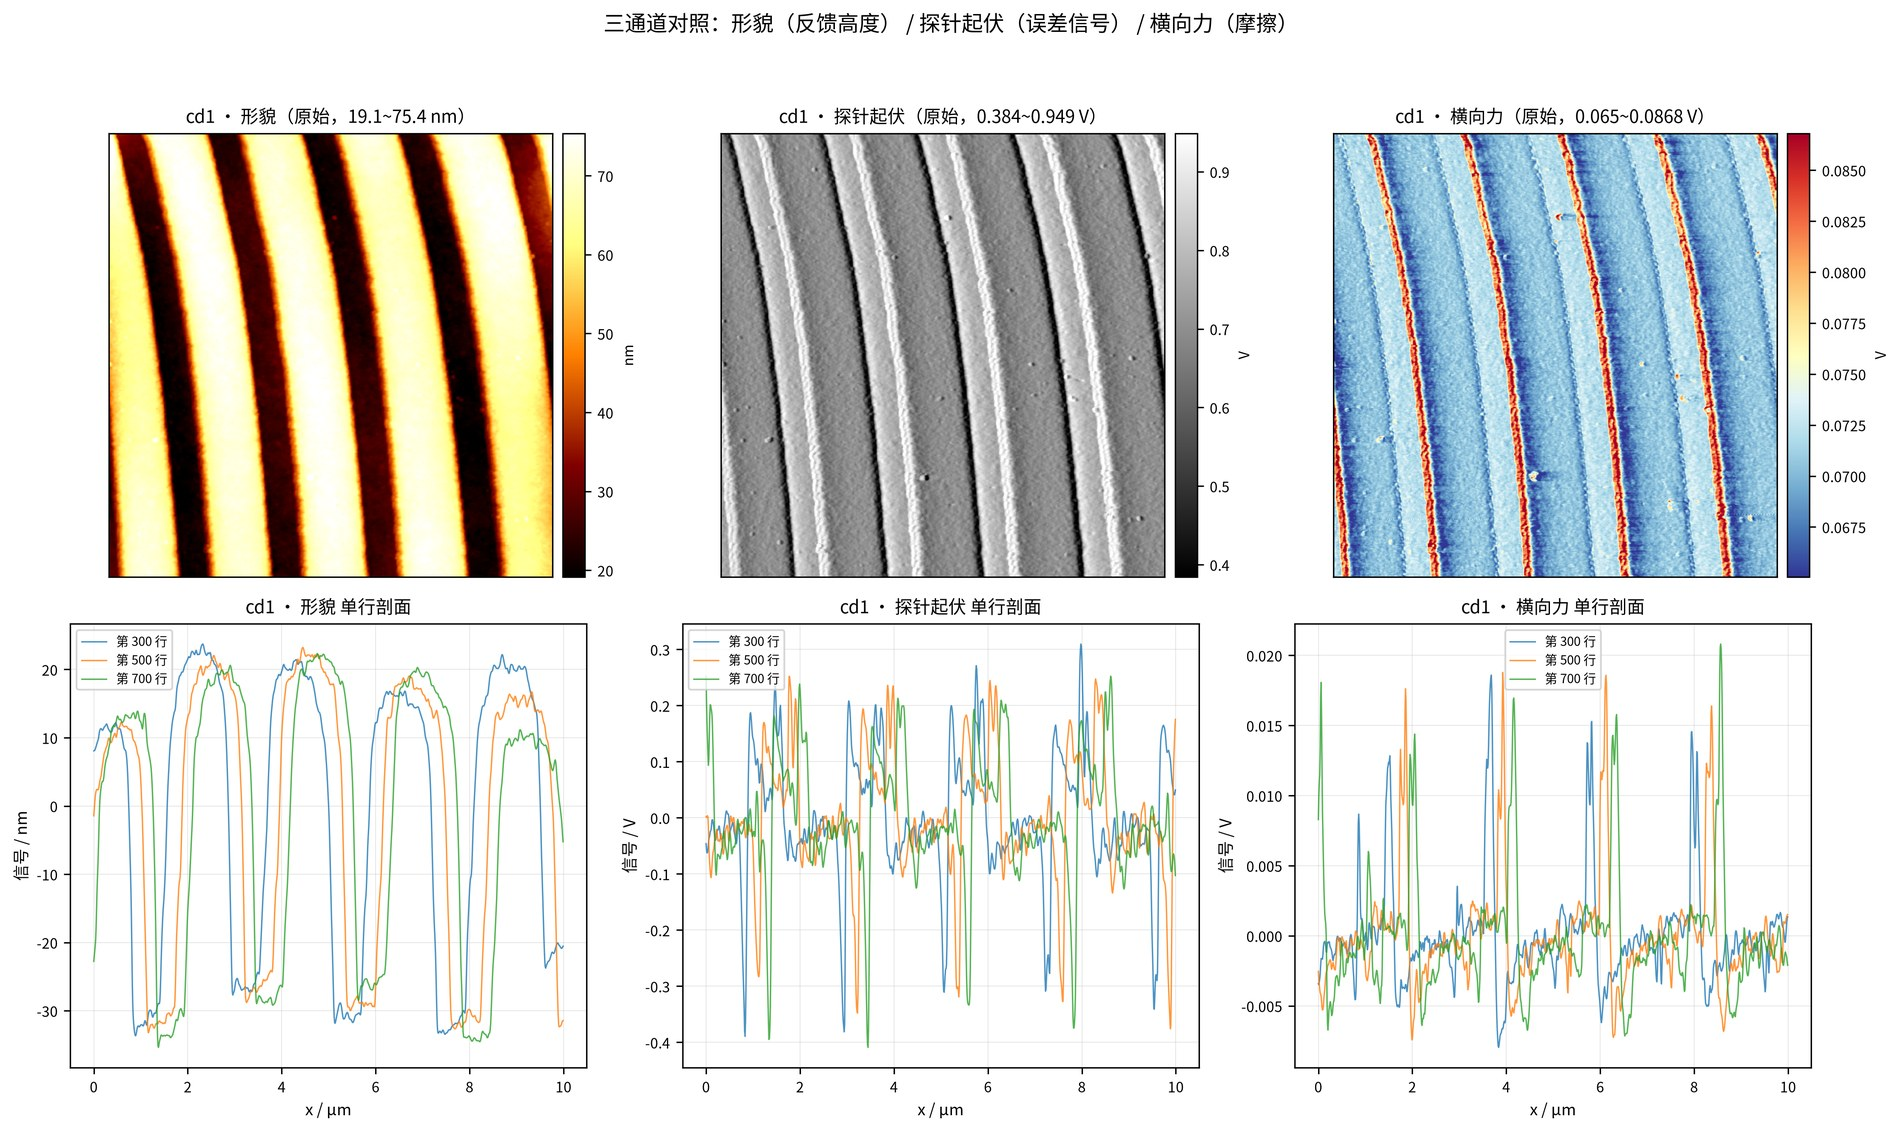
\includegraphics[width=0.95\textwidth]{fig06_channels.jpg}
\caption{cd1 的三通道对照。上排为原始图像（形貌、误差信号、横向力），下排为第 300、500、700 行的单行剖面。}
\label{fig:chan}
\end{figure}

\subsection{图像质量、伪迹与不确定度}

三组数据中未见扫描线伪迹。判据是原始图像的行均值序列：其标准差为 0.03--0.06~nm，相邻行均值差值的平均绝对值为 0.001--0.004~nm，单行最大 0.046~nm（出现在 cd2），而行内起伏的标准差在 20--31~nm。若存在反馈失锁或行间机械跳变，行均值会表现出与行内起伏同量级的突变，本数据中行均值无此类突变。这说明在 1.0~Hz 的扫描频率下，比例与积分增益取 200 时反馈回路对沟槽的高度变化有充分响应。

扫描器的压电非线性与迟滞是横向尺度的另一项系统误差。压电陶瓷的伸长量与驱动电压并非严格线性，文献把迟滞、蠕变与振动列为压电执行器定位精度损失的三条原因，并主张以逆模型补偿\cite{croft2001}；其表现是同一视场内不同位置的标定因子不同。第~\ref{sec:calib} 节对三张光盘各取一个标定因子，盘间差异为 6.9\%，跨盘的残余不一致为 7\% 量级，与该量级相当；若要进一步压低，需要在扫描范围内分区标定。

条纹倾斜是影响本批数据剖面幅度的主要伪迹，其来源是扫描轴与沟槽走向的实际夹角，而非测量误差；若不作行程对齐而直接沿慢扫方向平均，剖面幅度会被压低（cd3 由 88.6~nm 降至 8.1~nm），进而使“沟槽深度”的估计偏低一个量级。本文用相位斜率法统一估计并校正倾角，三组倾角分别为 $+8.1^\circ$、$0^\circ$ 与 $-13.2^\circ$。

探针卷积是深度读数的系统偏差来源。形貌图是表面与针尖形状的卷积：针尖比特征钝时，凸起被横向展宽、凹槽被压窄压浅\cite{lipeng2016}。周期读数不受这一效应影响：各周期的偏移方向相同，针尖卷积只改变谐波的幅度、不移动基频峰位。三次测量使用同一支探针，其型号与曲率半径未记录，无法给出确切值，只能给出量级判断：按手册对台阶的估计（半锥角 $10^\circ$ 时单边展宽约为台阶高度的 18\%\cite{manual_cspm}），以及槽壁对针尖的几何遮挡，实测深度应系统性小于真实槽深，而周期读数不受影响。

成像参数的对照受数据条件限制：三组数据在参考点（0.30）、扫描频率（1.0~Hz）、比例与积分增益（200/200）上完全相同，差别只在信号增益（7.0、7.0、5.0）、灵敏度（9.201、9.890、10.118）与满量程高度（105.28、105.28、147.39~nm）。因此本实验能提供的是“信号增益与满量程设置对成像的影响”，而不能单独考察扫描频率与参考点的作用；cd3 的结构最深，但其信号增益反而最低，说明这三组之间的形貌差异来自样品本身，而不是增益设置。扫描频率与参考点的作用需在同一样品上作单变量序列扫描才能分离，本实验未作这一序列。

% ============================================================
% 结论
% ============================================================
\section{结论}

本文用接触模式原子力显微镜测量了三张光盘的表面形貌，建立了从原始 \texttt{.csm} 文件到粗糙度与沟槽参数的完整处理链，主要结论如下。

（1）三张光盘的表面均由平行沟槽构成，周期分别为 $2170\pm4$、$2143\pm7$ 与 $1090\pm2$~nm，逐行峰谷深度分别为 55.2、60.4 与 93.4~nm，整平后面粗糙度 $S_q$ 为 20.26、19.94 与 31.02~nm。

（2）cd1 与 cd2 的周期在倾角修正后相差 0.25\%，属同一规格；以 CD 道距 1600~nm 为参照反推的扫描横向尺度因子为 1.34，据此 cd3 修正后周期为 792~nm，与 DVD 道距 740~nm 相差 7.0\%。三张光盘判为两张 CD 类与一张 DVD 类，该判断依赖外部型号确认，横向标定值本身不是本实验独立测得。

（3）条纹相对慢扫方向存在 $8.1^\circ$ 与 $-13.2^\circ$ 的倾斜，跨行平均前必须作行程对齐；未对齐时平均剖面的峰谷幅度可被低估约 11 倍（cd3 由 88.6~nm 降至 8.1~nm）。

（4）三组数据均无扫描线伪迹：行均值标准差不超过 0.06~nm，相邻行均值差的平均绝对值不超过 0.004~nm（最大 0.046~nm），说明在 1.0~Hz、增益 200/200 的条件下反馈回路稳定。

（5）二阶面整平对 $S_q$ 的改变不足 0.1\%，说明表面方差由条纹结构主导；偏度全为负、峭度均小于 3，表明表面为宽脊窄槽的平坦—陡壁交替结构。

（6）深度读数为真值的下限，探针卷积使槽型展宽、深度压缩；本实验探针型号未记录，无法定量修正。误差信号与横向力通道均与形貌通道同源，横向力在槽壁两侧呈反对称偏转，cd3 的相对幅度最大，与其结构最深、周期最短一致。

\section{意见与建议}

本次实验在数据采集之外的环节有三处可以改进。扫描器横向标定应作为独立环节先做：用已知周期的标准光栅按手册 §17.1 的流程标定 $X$、$Y$ 快慢扫四个方向，把标定因子作为已知量代入周期测量，而不以光盘道距反推。这样既能给出绝对尺度，也能暴露扫描器的非线性和各向异性（本机的快扫与慢扫伸缩系数相差 26.8\%，若标定不完整，图像在 $x$、$y$ 方向的尺度会系统不一致）。

样品与探针的信息应当记录。本实验三张光盘的型号与所用探针的曲率半径、锥角均未留下记录，导致周期只能作相对比较、深度无法作卷积修正。建议在采集时就登记盘片类型与探针批次，并在同一样品上补做扫描频率（0.5--3~Hz，覆盖手册推荐区间 1.0--2.0~Hz 的上下界）与参考点的单变量序列，这与第~1.4 节所列“比较处理前后参数的变化”与“定量评估伪迹对测量结果的影响量级”两项内容对应。

数据处理方面，建议把倾角估计与行列对齐作为标准步骤固定下来。本批数据中若沿用软件默认的“沿慢扫方向取剖面”，两张光盘的沟槽深度会被低估 46\%（cd1）与 91\%（cd3），而这一错误在剖面上表现为“起伏很小、沟槽不可辨”，很容易被误判为扫描失败。

% ============================================================
% 参考文献（条目顺序 = 正文首次引用顺序）
% ============================================================
\section{参考文献}
\renewcommand{\refname}{}
\setstretch{1.25}
\songti\zihao{5}
\begin{thebibliography}{99}

\bibitem{binnig1982}
Binnig G, Rohrer H, Gerber C, et al. Surface studies by scanning tunneling microscopy[J]. Physical Review Letters, 1982, 49(1): 57--61.
\url{https://doi.org/10.1103/PhysRevLett.49.57}

\bibitem{binnig1986}
Binnig G, Quate C F, Gerber C. Atomic force microscope[J]. Physical Review Letters, 1986, 56(9): 930--933.
\url{https://doi.org/10.1103/PhysRevLett.56.930}

\bibitem{giessibl2003}
Giessibl F J. Advances in atomic force microscopy[J]. Reviews of Modern Physics, 2003, 75(3): 949--983.
\url{https://doi.org/10.1103/RevModPhys.75.949}

\bibitem{mironov2004}
Mironov V L. Fundamentals of Scanning Probe Microscopy[M]. Nizhniy Novgorod: The Russian Academy of Sciences, Institute for Physics of Microstructures, 2004.

\bibitem{meyer1988}
Meyer G, Amer N M. Novel optical approach to atomic force microscopy[J]. Applied Physics Letters, 1988, 53(12): 1045--1047.
\url{https://doi.org/10.1063/1.100061}

\bibitem{garcia2002}
García R, Pérez R. Dynamic atomic force microscopy methods[J]. Surface Science Reports, 2002, 47(6--8): 197--301.
\url{https://doi.org/10.1016/S0167-5729(02)00077-8}

\bibitem{manual_cspm}
本原纳米仪器有限公司. CSPM5500 扫描探针显微镜系统用户手册（V1.11.10 中文版）[Z]. 2012.

\bibitem{kim1997}
Kim J S, Nam T Y, Huh Y J. The optical characteristics in the layers of compact disc-recordable[J]. Korean Journal of Chemical Engineering, 1997, 14(2): 88--92.
\url{https://doi.org/10.1007/BF02706066}

\bibitem{ecma394}
Ecma International. ECMA-394: Recordable compact disc systems --- CD-R multi-speed[S]. 1st ed. Geneva: Ecma International, 2010.
\url{https://ecma-international.org/wp-content/uploads/ECMA-394_1st_edition_december_2010.pdf}

\bibitem{ecma130}
Ecma International. ECMA-130: Data interchange on read-only 120 mm optical data disks (CD-ROM)[S]. 2nd ed. Geneva: Ecma International, 1996.
\url{https://ecma-international.org/wp-content/uploads/ECMA-130_2nd_edition_june_1996.pdf}

\bibitem{ecma267}
Ecma International. ECMA-267: 120 mm DVD --- read-only disk[S]. 3rd ed. Geneva: Ecma International, 2001.
\url{https://www.ecma-international.org/wp-content/uploads/ECMA-267_3rd_edition_april_2001.pdf}

\bibitem{bda2004}
Blu-ray Disc Founders. White paper: Blu-ray Disc format 1.A --- physical format specifications for BD-RE[S]. 2004.
\url{https://www.disc-group.com/wp-content/uploads/2011/05/Blu-Ray-1-PhysicalFormatSpecs-BD-RE-1.065KB.pdf}

\bibitem{sunjielin2001}
Sun J L, Zhang G X, Hu Q Q, et al. Applications of AFM technology in CD-R R\&D[C]//Proceedings of SPIE, 2001, 4085: 228--232.
\url{https://doi.org/10.1117/12.416848}

\bibitem{yanyg2005}
闫勇刚, 马强, 黄俊杰, 等. 基于 AFM 检测信息存储介质表面结构的研究[J]. 微纳电子技术, 2005(3): 139--141. \url{https://doi.org/10.13250/j.cnki.wndz.2005.03.010}

\bibitem{sunzhi2006}
孙志, 罗胜耘, 樊永发. 基于原子力显微镜的 CD/DVD 表面形貌检测[J]. 吉首大学学报（自然科学版）, 2006, 27(3): 55--56.

\bibitem{lipeng2016}
李鹏, 王朋伟, 刘竞艳, 等. 原子力显微镜形貌像的典型失真和伪迹[J]. 西安文理学院学报（自然科学版）, 2016, 19(1): 59--63.

\bibitem{hermes_agent}
Nous Research. Hermes Agent: an open-source AI agent system[CP/OL]. (2025)[\mbox{2026-10-27}]. \url{https://github.com/NousResearch/hermes-agent}

\bibitem{croft2001}
Croft D, Shed G, Devasia S. Creep, hysteresis, and vibration compensation for piezoactuators: atomic force microscopy application[J]. Journal of Dynamic Systems, Measurement, and Control, 2001, 123(1): 35--43.
\url{https://doi.org/10.1115/1.1341197}

\end{thebibliography}

% ============================================================
% 附录
% ============================================================
\newpage
\appendix
\section{数据处理流程与代码清单}

本文的全部数据处理由自编脚本完成，各脚本的功能与对应关系列于表~\ref{tab:code}，处理流程为：

\begin{enumerate}
  \item 解析 \texttt{.csm}：读取 BMP 头与像素区，按式~\eqref{eq:decode} 还原 16 位量并换算为 nm 或 V，解码末尾 GBK 参数块；
  \item 逐行一阶多项式拟合减除，消除行倾斜与行偏置；
  \item 全局二阶二维多项式拟合减除，完成面整平；
  \item 逐行一维傅里叶变换取主峰周期，取 1024 行的中位数与四分位区间；
  \item 逐行离散傅里叶变换的相位斜率法估计条纹倾角，按行插值平移后沿 $y$ 平均得平均剖面；
  \item 在平均剖面上取 $P_{99}-P_1$ 与占宽比，在整平后图像上按手册 §47.2 的参数定义计算面粗糙度；
  \item 计算一维功率谱与二维傅里叶谱，作三维形貌与各通道剖面图。
\end{enumerate}

\begin{table}[H]
\centering
\caption{数据处理脚本清单}
\label{tab:code}
\small
\setstretch{1.0}
\begin{tabularx}{\textwidth}{@{}lX@{}}
\toprule
脚本 & 功能 \\
\midrule
\texttt{csmio.py} & \texttt{.csm} 格式解析：BMP 头、像素反编码、参数块解码 \\
\texttt{afmproc.py} & 处理算子：逐行去倾斜、面整平、粗糙度、周期与倾角、功率谱 \\
\texttt{analyze.py} & 主流程：批量处理九个数据文件，输出参数表与数组 \\
\texttt{plot.py} & 出图：原始图像、处理链、剖面、频谱、三维形貌、通道对照 \\
\texttt{diag\_phase\_drift.py} & 逐行相位的线性/二次分解与分带局部倾角 \\
\texttt{diag\_phase\_factors.py} & 相位漂移四因素分解、曲率项注入-恢复标定与三种对齐方案比较 \\
\texttt{diag\_curvature\_2d.py} & 二维带通解调独立核验 $x$ 向曲率项 \\
\texttt{diag\_orientation\_tensor.py} & 结构张量分块法测局部条纹方向（独立核验）\\
\texttt{obs\_from\_csm.py} & 从原始 \texttt{.csm} 复算观测向量（周期、倾角、深度、帧内漂移）\\
\texttt{calib\_mcmc.py} & 贝叶斯联合拟合：仿射不变系综采样、四个模型的比较与后验汇总 \\
\bottomrule
\end{tabularx}
\end{table}

所有长度单位为 nm，高度由文件头的满量程高度换算，误差与横向力通道由满量程电压换算。原始数据、脚本与结果表已在 GitHub 公开（实验分支 \texttt{afm-cd-groove-morphology}）：

\noindent{\small\url{https://github.com/xzx-001/dlut-physical-exp}}

可用 \texttt{git clone -b afm-cd-groove-morphology} 取得，据此可复现本文全部数值。


\newpage
\section{面粗糙度参数的定义}
\label{app:sparam}

本文用到的八项区域法粗糙度参数按 Imager 手册 §47.2 的定义计算，评定面为 $10\,\mu\mathrm{m}$ 见方、$1024\times1024$ 点的整平后形貌。其中 $z$ 为相对评定面中值的高度，$\langle\cdot\rangle$ 表示在评定面上取平均，$A$ 为评定面面积，$N_{\text{peak}}$ 为局部峰个数，$z_{p,k}$ 与 $z_{v,k}$ 分别为第 $k$ 高的局部峰与第 $k$ 低的局部谷。其中 $S_z$ 取十点高度，与 ISO 25178 的同名参数（最大高度 $S_p+S_v$）不同；其余参数采用与 ISO 25178 同名参数相同的定义形式，具体定义式以手册 §47.2 为准。

\begin{table}[H]
\centering
\caption{面粗糙度参数的定义式与物理含义}
\label{tab:sparam}
\small
\setstretch{1.05}
\begin{tabularx}{\textwidth}{@{}l l l X@{}}
\toprule
符号 & 名称 & 定义式 & 物理含义 \\
\midrule
$S_a$ & 算术平均高度 & $\langle\lvert z\rvert\rangle$ & 起伏的平均幅度；与 $S_q$ 相比，它对少数深谷或高峰的权重更低，因而对孤立尖峰不敏感。 \\
$S_q$ & 均方根高度 & $\sqrt{\langle z^2\rangle}$ & 高度的标准差。平方加权使其对少数大起伏比 $S_a$ 敏感；是光学散射、接触刚度等模型的直接输入，也是最常用的单一比较量。 \\
$S_y$ & 最大高度差 & $\max z-\min z$ & 由单点极值决定，易受单个颗粒、毛刺或噪声尖峰的影响，重复性差，只宜作为上限参考。 \\
$S_z$ & 十点高度 & $\frac{1}{5}\sum\limits_{k=1}^{5}z_{p,k}-\frac{1}{5}\sum\limits_{k=1}^{5}z_{v,k}$ & 以局部极值替代单点极值，抗单点噪声，反映“典型峰—典型谷”的高差；数值上略小于 $S_y$。 \\
$S_{sk}$ & 偏度 & $\langle z^3\rangle/S_q^3$ & 高度分布的三阶归一化矩。零为对称；负值表示谷窄而深、脊宽而平（与占宽比大于 0.5 的“宽脊窄槽”剖面一致）；正值为尖峰多。 \\
$S_{ku}$ & 峭度 & $\langle z^4\rangle/S_q^4$ & 四阶归一化矩。高斯分布取 3；小于 3 表示分布比正态平坦、表面以平台为主；大于 3 表示起伏集中在少数尖峰与深谷。 \\
$S_{dq}$ & 均方根斜率 & $\sqrt{\big\langle(\partial z/\partial x)^2+(\partial z/\partial y)^2\big\rangle}$ & 局部坡度的典型陡缓，单位弧度。梯度按像素间距计算，跨仪器比较时须换算到同一像素尺度。 \\
$S_{ds}$ & 峰密度 & $N_{\text{peak}}/A$ & 纹理在横向的疏密（单位 $\mu\mathrm{m}^{-2}$）：周期越短，单位面积内的脊条越多，峰密度越高，近似与周期成反比。 \\
\bottomrule
\end{tabularx}
\end{table}

\end{document}
